\documentclass{article}
\usepackage[utf8]{inputenc}
\usepackage[margin=1in]{geometry}
\usepackage{graphicx}
\usepackage{nth}
\usepackage{amsmath}
\usepackage{mathtools}
\usepackage{siunitx}
\usepackage{bm}
\usepackage{enumitem}
\usepackage{hyperref}
\usepackage{amssymb}
\usepackage{soul, color}
\usepackage[cc]{titlepic}
\usepackage{float}
\hyphenpenalty 10000
\usepackage[sorting=none, backend=biber]{biblatex}
\addbibresource{reportbib.bibtex}
% \setcounter{biburllcpenalty}{7000}
% \DeclareMathOperator{\erf}{erf}
\renewcommand*\footnoterule{}

\title{Advanced Bayesian Data Analysis for \\ Astrophysics, Cosmology and Beyond}
\author{Adam Ormondroyd\\ \\Supervisors: Prof.~M.P.~Hobson, \\ Dr.~W.J.~Handley, Prof.~A.N.~Lasenby\\ \\Cavendish Astrophysics}
\date{July 2022}

\begin{document}
\setcounter{page}{0}
\maketitle

\begin{figure}[!h]
  \centering
  
\includegraphics[width=5cm]{University_Crest.pdf}
  \label{fig:crest}
\end{figure}

\begin{abstract}

In cosmology, there are many cases where it is useful to reconstruct one--dimensional functions, such as the primordial matter power spectrum or how the dark energy equation of state parameter changes with redshift. The most general approach would be to fit a free--form function, where the nature of the function is itself determined by the data, not just its parameters. One such approach to this is to use a \textit{linf}: a linear spline between a variable number of nodes. This problem requires exploring a highly degenerate and multi--modal posterior distribution: nested sampling is a natural tool to investigate this.

For the first year of my PhD, I have focussed on learning how to use existing code: the cosmological Boltzmann code \texttt{CAMB}, the sampling and modelling framework \texttt{Cobaya}, and the nested sampler \texttt{PolyChord}.

I begin by exploring toy examples with \texttt{PolyChord}, then move to reconstructing the primordial matter power spectrum. This exposes an issue with \texttt{PolyChord} where it fails to identify clusters of sampling live points at higher resolution and therefore misses a posterior mode present at lower resolution. Dr.~Handley and I add an interface to \texttt{PolyChord} to enable the user to provide a custom clustering algorithm, and plan to investigate alternatives to \texttt{PolyChord}'s native K--nearest--neighbours method.

The distribution version of \texttt{Cobaya} only allows the user to provide their own $\mathcal P_\mathcal R(k)$ function for the primodial matter power spectrum. To investigate the dark matter equation of state, I add an interface to \texttt{Cobaya} to allow $w(a)$ to be provided in a similar way. This interface is almost ready, except for the need for \texttt{Cobaya} to automatically understand that the equation of state parameters can be sampled together with the other \texttt{CAMB} parameters.
\end{abstract}

\newpage

\tableofcontents

\newpage

\section{Introduction}
This report summarises the first year of my PhD. I have focussed primarily on familiarising myself with existing code, in particular the cosmology code \texttt{CAMB} (Code for Anisotropies in the Microwave Background) \cite{CAMB_1, CAMB_2}, the sampling and modelling framework \texttt{Cobaya} (\textbf{Co}de for \textbf{bay}esian \textbf{a}nalysis) \cite{Cobaya}, and the nested sampler \texttt{PolyChord} \cite{PolyChord_1, PolyChord_2}. The theme has been to use a \textit{linf}, a linear spline between either a fixed or variable number of nodes, to reconstruct a function from data.

I began by exploring toy examples with \texttt{PolyChord}, then proceeded to apply this to cosmology. I reconstructed the primordial matter power spectrum, using the interface which \texttt{Cobaya} provides. This revealed an issue with \texttt{PolyChord}, where the native K--nearest--neighbours clustering fails to identify separate clusters of parameters at higher resolutions. I have worked with Dr.~Handley to add an interface to \texttt{PolyChord} where the user can supply their own Python clustering, so that we will be able to experiment with different algorithms.

The primordial matter power spectrum was practice for reconstructing the dark energy equation of state parameter $w$ in the same way, which is more difficult as \texttt{Cobaya} does not provide an interface for this. I have added this myself, which is working and almost finished, but I cannot make any conclusions about dark energy until the issues with \texttt{PolyChord} have been resolved. 

\section{Cosmological Context}
\label{sec:context}
\subsection{Cosmological tensions}
The expansion of the universe if characterised by the Hubble parameter $H(t)=\dot{a}/a$, where $a$ is the cosmological scale factor, and its value today, the famous Hubble constant $H_0 \coloneqq H(\textrm{today})$. The ``Hubble tension'' is the famous descrepency between values of $H_0$: Planck collaboration measures a value of $H_0=67.4$ \unit{km.s^{-1}.Mpc^{-1}} from the early universe, while the SH0ES team finds $H_0=73.2$ \unit{km.s^{-1}.Mpc^{-1}} using distance ladders. If this ``Hubble tension'' is not due to systematic error, then the $\Lambda$CDM cosmological model may be somehow incomplete \cite{buyers-guide}.

Another cosmological tension is the ``$S_8$'' tension. Weak galaxy lensing surveys consistently favour a lower amplitude for matter fluctuation spectrum than expected by $\Lambda$CDM at low redshifts, $z\gtrsim 0.5 \hyphen 1$. The matter fluctuation spectrum is quantified by the parameter $S_8 \coloneqq \sigma_8 \sqrt{\Omega_\textrm m / 0.3}$. $\sigma_8$ is the root--mean--square matter fluctuation over a sphere of radius $8h^{-1}$ \unit{Mpc^{-1}}, where $h$ is the Hubble constant's dimensionless cousin ($H_0=100 h$ \unit{km.s^{-1}.Mpc^{-1}}) \cite{s8-drag}. These measurements can also be reconciled with Planck $\Lambda$CDM cosmology, for example by modifying the matter power spectrum on non-linear scales \cite{Amon-2022}.

\subsection{Existing dark energy parameterisations}

A useful general approach in cosmology is reconstructing one--dimensional functions, prime examples are the primordial matter power spectrum $\mathcal P_\mathcal R(k)$, and the equation of state parameters of various ideal fluids $w(a)$, such as dark matter or dark energy. Historically, this has been achieved by assuming a particular functional form, in the case of the power spectrum it is usually written as a power law $\log{\mathcal P_\mathcal R} \propto \log{k}$. In lieu of a theoretical understanding of dark energy, a number of dark energy equation of state parameterisations exist, for example \cite{Vazquez_2012}:

\begin{equation}
  w(a) = 
  \begin{cases}
  = w_0 \qquad & \textrm{(cosmological constant)} \\
  = w_0 + (1-a) w_a \qquad & \textrm{(CPL)}\\
  = w_0 + (1-a)a w_a \qquad & \textrm{(JBP)}\\
  = w_a + (w_0-w_a) \frac{a^{1/\tau}[1-(a/a_t)^{1/\tau}]}{1-a_t^{-1/\tau}} \qquad & \textrm{(FNT),}\\
  \end{cases}
\end{equation}
%
which are the constant, Chevallier--Polarski--Linder (CPL) \cite{CPL_1, CPL_2}, Jassal--Bagla--Padmanabhan (JBP) \cite{JBP}, and Felive--Nesseris--Tsujikawa (FNT) \cite{FNT} parameterisions, to name a few.

Assuming a particular functional form has limitations, ideally the data should be able to demand structure where it needs it, and simplicity where it doesn't --- a ``free--form" reconstruction. One such reconstruction is a linear spline between nodes in $(a, w)$ space, where the number of nodes is itself a parameter to be determined. This is not totally free--form, but freer than most, as the data is free to choose the level of complexity.

The linear spline is an appropriate choice as an appeal to simplicity. If we perform a polynomial spline between all nodes, then the requirement of continuous first and second derivatives can lead to nodes having tight error bars while lying nowhere near the original function. For example, suppose a three-node reconstruction of $f(x)$ is well constrained at low and medium $x$, but less so at large $x$. As the positions of the left and intermediate node will be well constrained, they will influence the position of the right node, attributing it a lower uncertainty than appropriate. This is not desired, the choice of polynomial has directly influenced the position and uncertainty of a node, which is at odds with a free--form approach. Therefore, a linear spline is a better description \cite{Vazquez_2012_pk}. Dark energy exists as a postulate to explain the late--time acceleration of the universe's expansion, therefore the most minimal assumptions about its dynamical behaviour must be made and tight derivative constraints would be directly at odds with this.

An alternative and currently popular approach might be to use a Gaussian Process regression. This approach makes the assumption that both the data and the function being reconstructed are Gaussian, and their distribution can be fully described by a mean function and a covariance kernel. The choice of mean function is important, and is neglected in a lot of the literature, which typically uses zero as the mean function \cite{GP}. This choice again contradicts our desire for simplicity, and faces a similar condition to a polynomial spline in that the derivative must also conform to a Gaussian distribution.

Fitting a linear spline with a variable number of nodes is a self--consistent approach which uses Bayesian methods to constrain both the number of parameters and their values. The posterior is therefore multi--modal and degenerate, as extra nodes can always be inserted without changing the function, and more than one mode may exist for a given number of nodes, such as those seen in section \ref{sec:polychord_revisited}. Nested sampling is a natural tool to investigate such a problem, and I will focus on the \texttt{PolyChord} implementation.

\subsection{Related work in the group}
\label{sec:barker}
If dark matter and dark energy indeed exist, it would seem natural that a ``dark radiation'' would also exist to mediate the interactions between such particles \cite{Ackerman_2009}. A transision in the behaviour of this radiation has the potential to answer the Hubble tension \cite{Aloni_2022}. Theoretical work by Dr.~Barker, another member of the group, provides a gravitational mechanism for this \cite{Barker_2020}. This work explores a one-parameter extension to $\Lambda$CDM, an effective dark radiation which tracks the dominant equation of state parameter of the current epoch: 

\begin{equation}
  w_\textrm{eff} = 
  \begin{cases}
    \begin{aligned}
      w_\textrm{r,eff} &= 1/3 \\
      w_\textrm{m,eff} &= (1-1/\sqrt{3}) / 2 \approx 0.211 \\
      w_{\Lambda \textrm{,eff}} &= 1/\sqrt{3} \approx 0.577 \textrm{.} \\
    \end{aligned}
  \end{cases}
\end{equation}

Within gravity, the Lagrangian may contain invariants of the field strengths up to second order. The Einstein field equations arise from varying from the Einstein-Hilbert action:

\begin{equation}
  \label{eq:einstein-hilbert}
  L_\textrm T = \frac{1}{2\kappa}R - \frac{\Lambda}{\kappa} + L_\textrm M
\end{equation}
%
where the gravitational portion $L_\textrm G = L_\textrm T - L_\textrm M$ is powered by the Riemann curvature, $R \equiv {R^{\mu\nu}}_{\mu\nu}$. The matter lagrangian $L_\textrm M$ provides the standard model of particle physics when below the electroweak transition temperature. Two physical scales are expressed, identified by the Einstein constant $\kappa=8\pi G$ and the cosmological constant $\Lambda$. 

Barker /cite{barker-thesis} notes that, had the standard model predated general relativity, the theoretical minimalism of the Einstein--Hilbert action might have been called into question as it lacks quadratic terms. For example, the electromagnetic lagrangian density:

\begin{equation}
  \mathcal L_\textrm{EM} = -\frac{1}{4} F_{\mu\nu}F^{\mu\nu} + j_\mu A^\mu \textrm .
\end{equation}

Barker uses Poincar\'e gauge theory (PGT), which gauges rotational, translation, and torsional fields to find an alternative to \ref{eq:einstein-hilbert} constructed entirely from quadratic invariants of the Riemann-Cartan curvature $\mathcal R^{ijkl}$ and the torsion $\mathcal T^{ijk}$:

\begin{equation}\begin{aligned}
  \label{eq:lagrangian}
  L_\textrm G = & -\frac{4}{4\kappa}\mathcal T_i\mathcal T^i - \frac{\hat{\alpha}_6}{6} [\Lambda\mathcal T_{ijk}(\mathcal T^{ijk}-2\mathcal T^{jik}) \\ & + \mathcal R_{ij}(\mathcal R ^{[ij]}-12\mathcal R^{ij}) - 2\mathcal R_{ijkl}(\mathcal R ^{ijkl}-4\mathcal R^{ikjl}-5\mathcal R^{klij})] + 2\hat{\alpha}_5\mathcal R_{[ij]}\mathcal R^{[ij]} \textrm{.}
\end{aligned}\end{equation}

The Einstein--Hilbert term has been replaced by the the square of the torsion contraction $\mathcal T_i \equiv \mathcal T^j_{ij}$, which self-couples with strength $\kappa$. The cosmological constant $\Lambda$ is also a torsion self-coupling, rather than parameterising a mysterious energy density. The values of the dimensionless self-coupling constants $\hat\alpha_5$ and $\hat\alpha_6$ are not determined, but with the conditions
\begin{equation}
  \Lambda > 0,\quad \hat\alpha_6<0,\quad (\hat\alpha_5+2\hat\alpha_6)(\hat\alpha_5-\hat\alpha_6) > 0 \textrm{,}
\end{equation}
%
the linearisation of \ref{eq:lagrangian} on a matter--free, flat and torsionless background is power--counting renormalisable, unitary, and free from ghosts and tachyons. Ghosts are unphysical states in a gauge theory, which would be necessary if the local fields exceed the number of physical degrees of freedom. An example of a ghost exists in electromagnetism: one uses a four-vector potential $A_\mu(x)$, while the photon only has two polarisations \cite{Faddeev:2009}. Tachyons are particles that travel faster than light \cite{tachyon}.

Equation \ref{eq:lagrangian} produces the same cosmology as \ref{eq:einstein-hilbert}, but also allows a deviation from the vacuum expectation value which masquerades as dark radiation - a possible solution to the Hubble tension.


\section{Computational Context}
\subsection{Bayes' theorem}
Inductive logic, also known as plausible reasoning, is the problem faced by most scientists. Given that a certain set of effects have been observed, what model would have best predicted these? This is as opposed to the deductive logic usually employed in pure mathematics, and is typically a greater challenge. \cite{skilling}

Starting from Cox's rules of probability one arrives at Bayes' theorem \cite{Sivia2006}:

\begin{equation}
  \Pr({B|A}) = \frac{\Pr(A|B)\Pr(A)}{\Pr(B)} \textrm,
\end{equation}
%
for events $A$ and $B$. This can be framed as \textit{``updating the prior''}:
\begin{equation}
  \label{bayes-simple}
  \textrm{Posterior} = \frac{\textrm{Likelihood} \times \textrm{Prior}}{\textrm{Evidence}} \textrm .
\end{equation}

The prior represents the knowledge of the parameters of a model, before undertaking an experiment. The likelihood is the probability of observing the results of that experiment, given a set of parameters. The evidence, also known as the global likelihood, is the numerator of \ref{bayes-simple} marginalised over all possible parameters, and therefore normalises the expression. The posterior is then the updated knowledge of the parameters following the experiment.

Evaluating the evidence represents the key challenge of Bayesian analysis, and one must turn to numerical methods to evaluate the high-dimensional integral. 

\subsection{Numerical integration for evidence calculations}
Numerical integration techniques in general could fill several reports by itself, so I will restrict discussion to techniques used in cosmological evidence calculations.

A Monte Carlo algorithm is a randomised algorithm, whose result will differ from the true result with known probability. Unlike deterministic approaches such as trapezoid rule, Monte Carlo algorithms are non-determministic. Monte Carlo integration uses the approximation

\begin{equation}
\int_\Omega f(x) dx \approx V \frac{1}{N}\sum_{i=1}^{N} f(x_i) \textrm .
\end{equation}
%
$V$ is the volume of the integration domain $\Omega$. Monte Carlo integration methods then differ by how the samples $x_i$ are generated. The most vanilla Monte Carlo integration simply draws samples at random from $x$. This algorithm is at risk of missing small regions of $\Omega$ containing large contributions to the integral, which is the case for most high-dimensional integrals. This can be improved using importance sampling: drawing samples from a probability distribution which weighted towards the regions of high $f$. Markov chain Monte Carlo (MCMC) starts with a random point, and a Markov chain is constructed from it. There are many algorithms for constructing the chain, Metropolis Hastings, Gibbs sampling, slice sampling, to name a few. 

As the number of dimensions increases, MCMC can too suffer from the ``curse of dimensionality'' it was designed to avoid. Shortening the Markov steps can help, but this leads to highly autocorrelated samples, so more samples are needed, and would therefore need to run for longer. MCMC is also not trivially parallelisable, aside from running multiple chains in parallel, which can be used to assess convergence. In cosmological applications, where the greatest computational cost is the generation of a new point, a different approach is needed: nested sampling.


\section{Nested Sampling}
\subsection{The idea}
Nested sampling is an algorithm developed by John Skilling for calculating the evidence $Z$, the probability of data given a particular model \cite{skilling} \cite{Ashton_2022}. Posterior samples are an optional by--product. This is typically in the context of Bayes theorem:
\begin{equation}
  \textrm{Posterior} = P = \Pr\left(\bm{\theta}| D, \mathcal{M}\right) = \frac{\Pr\left(D|\mathcal{M}(\bm\theta)\right) \times \Pr\left(\bm\theta\right)}{\Pr\left(D|\mathcal{M}\right)} = \frac{\textrm{Likelihood} \times \textrm{Prior}}{\textrm{Evidence}} = \frac{L(\bm\theta) \pi(\bm{\theta})}{Z}\textrm,
  \label{bayes}
\end{equation}
%
for a model $\mathcal{M}$ and its parameters $\bm{\theta}$. The evidence Z is used to compare models $\mathcal{M}_i$ and $\mathcal{M}_j$ through the Bayes factor and posterior odds ratio:

\begin{equation}
  \mathcal{P}_{i, j} = \ln\frac{\Pr\left(D|\mathcal{M}_j\right)}{\Pr\left(D|\mathcal{M}_i\right)}
  \mathcal{B}_{i, j} = \mathcal{B}_{i, j} + \ln\frac{\pi_{\mathcal{M}_i}}{\pi_{\mathcal{M}_j}} \textrm, \quad \mathcal B_{i, j} \coloneqq \ln\frac{Z_i}{Z_j} \textrm,
\end{equation}
%
where $Z_i$ is the evidence of model $\mathcal M_i$. The posterior odds is perhaps a more complete assessment of the relative performance of two models, but the Bayes factor is more common in the literature \cite{Sonke}. The models I consider have equal priors, so $\mathcal{P}_{i,j} = \mathcal{B}_{i,j}$ \cite{Sonke}.

The Bayesian evidence is the normalisation of the numerator in Bayes' theorem, so in theory can be calculated by numerical integration. This becomes impractical to solve using typical numerical integration techniques, such as rastering over $\bm\theta$, once $\bm\theta$ has many dimensions. Instead, define an element of prior mass, $dX = \pi(\bm\theta)d\bm\theta$. $X$ can be accumulated from $dX$ in any order, so by defining:
%
\begin{equation}
  X(\lambda) = \int_{L(\bm\theta)>\lambda} \pi(\bm\theta)d\bm\theta\textrm,
\end{equation}
%
i.e.\ $X$ is the cumulative prior mass for likelihood greater than $\lambda$. The evidence then becomes a one-dimensional integral:
%
\begin{equation}
  Z = \int_0^1 L(X) dX\textrm,
\end{equation}
%
where $L(X(\lambda)) = \lambda$. This transformation requires sorting the prior mass elements by likelihood. Given the set of $m$ points:
\begin{equation}
  0<X_m<\dots<X_2<X_1<1, \quad L_i = L(X_i)\textrm,
\end{equation}
%
a sensible numerical recipe would estimate $Z$ as a weighted sum:
%
\begin{equation}
  Z \approx \sum_{i=1}^m w_i Z_i\textrm.
\end{equation}
%
Because $L(X)$ is monotonically decreasing, it must be larger than any value at larger $X$, so $w_i=X_i-X_{i+1}$ gives a lower bound. As it must also be smaller than any value at smaller $X$, $X_{i-1}-X_i$ provides an upper bound:

\begin{equation}
  \sum_{i=1}^m (X_i-X_{i+1})L_i \le Z \le \sum_{i=1}^m (X_{i-1}-X_i)L_i + X_mL_\textrm{max}\textrm.
\end{equation}
%
$L_\textrm{max}$ is the maximum likelihood value found as $X\to0$. A tiny volume containing huge likelihood could always exist, and as such $L_\textrm{max}$ cannot be determined by any kind of sampling.
 
$Z$ is dominated by the region of bulk posterior mass. This typically occupies a fraction $e^{-H}$ of the prior, where:
%
\begin{equation}
  H = \textrm{information} = \int \log\left(dP/dX\right)dP\textrm.
\end{equation}
%
$H$ can be the order of thousands in practical problems. By considering the likelihood to consist of $C$ principal components, the posterior mass is expected to be broadly distributed over $-H\pm\sqrt{C}$ in $\log X$. Each principal component significantly restricts the range permitted by the prior, so $H$ should usually exceed $C$, which suggests that finding the posterior domain is more difficult than navigating within it. Therefore, to cover such a range, sampling should be linear in $\log X$ rather than $X$, so instead set:

\begin{equation}
  X_1 = t_1, X_2 = t_1t_2, \dots, X_m = t_1t_2t_3\dots t_m, 0<t_i<1\textrm.
\end{equation}
%
It is not usually possible to set precise values of $t$, but setting them statistically is enough. At each step, we need to find a new $X_i$ from the prior, subject to $X_i = t_i X_{i-1}<X_{i-1}$. The knowledge of this new point is specified by drawing $t_i$ from $\textrm{Uniform}(0, 1)$. This could be obtained by:
\begin{enumerate}
  \item sampling $X_i$ uniformly from the range $[0, X_{i-1}]$ then using the original likelihood sorting to find its corresponding $\bm\theta_i$, or
  \item sample $\bm\theta$ directly subject to $L(\bm\theta)>L_{i-1}$ in proportion to the prior.
\end{enumerate}

These methods are equivalent, but (b) does not use the prior mass, so the sorting step is not needed.

\subsection{Nested sampling algorithms}

Several variants around Skilling's original nested sampling algorithm exist. In general, the posterior will be multi-modal, and is dealt with in different ways in different algorithm. 

\begin{itemize}
  \item \texttt{MultiNest}, developed by Prof.~Hobson and Dr.~Faroz, constructs a series of overlapping ellipsoids around the live points to approximate the isolikelihood contour. Multi--modal posteriors will cause the ellipsoids to separate, at which point the modes can be identified and evolved independently. 
  \item \texttt{PolyChord} uses slice sampling to navigate the isolikelihood contour. It applies a clustering algorithm to the live points to identify posterior modes, so that each can be ``whitened'' independently. The modes then evolve semi-independently. \texttt{PolyChord} is discussed further in sections \ref{sec:poly} and \ref{sec:polychord_revisited}.
  \item Dynamic nested sampling differs from traditional nested sampling by using a dynamic number of live points. This can yield greater number of posterior samples for the same computational cost of traditional nested sampling. \texttt{dyPolyChord} and \texttt{dynesty} implement this by beginning with a traditional run with a small number of live points. The algorithm then calculates the importance of each sample, then finds the first ($j$) and last ($k$) live points with greater than a fraction (default 0.9 in \texttt{dyPolyChord}) of the greatest importance. Nested sampling is then repeated with more live points, starting at likelihood $L_{j-1}$ and finishing with the first sample taken with likelihood greater than $L_{k+1}$. This process is repeated until a termination condition is reached. The initial number of live points must be large enough to discover all modes of the posterior, as any modes with a maximum likelihood greater than $L_{k+1}$ will not be explored properly. Therefore, it may be unsuitable for the applications discussed here, which are highly multi--modal. \texttt{PolyChord} also implements dynamic nested sampling, but puts responsibility on the user, who must provide a function $n_\textrm{live}(L)$. Similarly, this function would be calculated using an initial low--resolution run. The low--$n_\textrm{live}$ parts of the run will contribute larger Poisson error to the volume estimate, and therefore the evidence calculation. In practice, normal nested sampling provides plenty of posterior samples, so aside from very specific applications, dynamic nested sampling is unnecessary.
\end{itemize}


\subsection{PolyChord}
\label{sec:poly}
\texttt{PolyChord} is a nested sampling algorithm developed by my supervisors Dr.~Handley, Prof.~Hobson and Prof.~Lasenby \cite{PolyChord_1, PolyChord_2}. It is distinguished from historical implementations in how it performs the final part of the iterative step, drawing a new point from the prior subject to $L(\bm\theta)>L_{i-1}$. Skilling orignally envisaged a Markov-Chain procedure, taking steps according to a proposal distribution until an independent sample is produced. These intermediate ``phantom" points have the potential to yield more information.

\texttt{PolyChord} uses slice sampling to sample within the isolikelihood contours. To slice sample, first choose a probability level ``slice" $P_0$ within $[0, P_\textrm{max}]$, then sample uniformally within the parameter space $P(\bf\theta)>P_0$. \texttt{PolyChord} adds features atop Aitken and Akman's slice-based nested sampling. It uses information present in both the live and phantom points to deal with correlated posteriors, and a clustering algorithm to identify separate posterior modes and evolve them semi-independently, calculating local evidences for each of them. It also has the option to implement fast-slow parameters, which is effective when sampling cosmologies.

The \texttt{PolyChord} algorithm is written in FORTRAN, and parallelised using \texttt{OpenMPI}. \href{https://github.com/PolyChord/PolyChordLite}{\texttt{PolyChordLite}}\footnote{\href{https://github.com/PolyChord/PolyChordLite}{https://github.com/PolyChord/PolyChordLite}} uses C++ to provide a Python interface, which I have used exclusively for my cosmological work. It is optimised for the case where runtime is dominated by the cost of generating new live points. This is frequently encountered in cosmology, due to the high dimensionality and costly likelihood evaluation.

\subsection{Slice sampling}

For each iteration $i$ of nested sampling, a point within the iso--likelihood contour $L_i$ is generated. This sampling is performed in the unit hypercube, with coordinate $\bm x$. One of the live points is chosen at random as a start point for a new chain, with coordinate $\bm x_0$. A step is then taken in the direction $\hat{\bm n}_0$ with distribution $P(\hat{\bm n})$ with width $w$, to generate the point $\bm x_1$. This is repeated $n_\textrm{repeats}$ times.

\texttt{PolyChord} uses the covariance matrix $\Sigma$ of the set of live and phantom points to infer the size and shape of the iso-likelihood contour, and determine an optimal $P(\hat{\bm n})$ and $w$. Uniformly transformed points remain so after an affine transformation:

\begin{equation}
  \textrm{L}^{-1}\bm x = \bm y,\qquad \textrm{LL}^{\intercal} = \Sigma\textrm,
\end{equation}
where $\textrm{L}$ is the Cholesky decomposition of the covariance matrix. The new space containing $\bm y$ is termed the ``sampling space". This transformation gives the contour size $\mathcal{O}(1)$ size in every direction, ``whitening" it, so $w=1$ is a suitable initial step size. 
$P(\hat{\bm n})$ is inspired by CosmoMC, which chooses a randomly oriented orthonormal basis, uses these directions in a random order, and generates a new one when this is exhausted \cite{CosmoMC}.

\subsection{Clustering}

The following step in nested sampling is clustering. A multi--modal distribution cannot be explored properly without grouping live points by their separate iso--likelihood contours, and exploring each mode independently. These modes are identified by the clustering of live points. Performing this at every iteration would add a large overhead to the calculation; in practice checking every $\mathcal{O}(n_\textrm{live})$ iterations is enough, as the live points will have compressed only by a factor of $e$ \cite{PolyChord_1}. The algorithm must be capable of identifying the number of clusters, as this is unknown. \texttt{PolyChord} uses a recursive variant of the K--nearest--neighbours, which satisfies this property. In principle, any such clustering algorithm should be sufficient, as the conditions of nested sampling mean there is no noise as each of the live points will be in exactly one of the iso--likelihood contours. When a live point dies, the new live point may appear in any of the surviving clusters, weighted by the prior volume of each cluster. A cluster dies when it contains zero live points.

\subsection{Interpreting results}

I have used the Python packages \texttt{anesthetic} for reading nested sampling chains into Python and producing posterior plots, and \texttt{fgivenx} for producing the functional posterior plots \cite{anesthetic, fgivenx}. The functional posterior plots produce a plot of some function $f(x, \bm\theta)$ marginalised over the posterior samples of $\bm\theta$. Examples of this are shown in figures \ref{fig:toysineadaptive}, 
\ref{fig:Pk_vanilla_100}, \ref{fig:N3} and \ref{fig:externalwa}. This provides more insight than simply plotting $f$ for the ``best fit" $\bm\theta$, as there might exist different modes of solutions that would otherwise be missed.

\hl{Suspiciousness}

Models are often compared using the 

\section{Toy Examples}
\label{toyexamples}
To develop my understanding of \texttt{PolyChord}, I repeated the work by S.~Hee et al.\ \cite{Sonke} This work uses linear splines as empirical models whose parameters are found using \texttt{PolyChord}, beginning with two toy datasets. One is $\sin\left({x/2\pi}\right)$ plus Gaussian noise, the other a ``line" wave, consisting of straight lines passing though $(1/4, 1)$ and $(3/4, -1)$ with period $1$. I added a third ``flat" case, replacing the line or sine with zero. For each case, I considered both errors in just the $y$--coordinate, and in both $x$ and $y$. A \textit{linf} can represent the line and flat cases exactly with $N=1$ and $N=4$ respectively.

To create each dataset $\left\{x_i, y_i\right\}$, 50 $x$--coordinates were drawn uniformly from $\left[0, 1\right]$, to which I applied one of the three functions to give the $y$--coordinate, and finally added homoskedastic Gaussian noise with $\sigma = 0.05$ in either just the $y$ or both directions. Any points taken out of $0\leq x < 1$ by the noise were deleted. My code is also vectorised to handle heteroskedastic errors.

Two types of linear spline are used. The first is a ``vanilla" linear spline which consists of $N$ nodes, labelled $0$ through $N-1$. The nodes must be sorted in increasing $x$--coordinate, the end nodes ($0$ and $N-1$) have fixed $x$--coordinate, but are otherwise free to move. The second is an ``adaptive" linear spline. $N$ is instead a parameter, which controls the number of nodes to use out of a maximum $N_\textrm{max}$. For example, if $N=5$ and $N_\textrm{max}=8$, nodes 0, 1, 2, 3, and 4 are treated as normal, but node 4 is connected directly to node 7, ignoring 5 and 6. If $N=1$, then the spline is constant at the height of the {$N-1^\textrm{th}$} node. This is an example of a nested model; vanilla splines with $N$ ranging from 1 to $N_\textrm{max}$ are nested with each other. In practice, \texttt{PolyChord} sees $N$ as a continuous parameter which is then rounded down. Note that the $N$ used in this and S.~Hee's work is different, here it refers to the total number of nodes, as opposed to the number of internal nodes.

These two splines allow two different approaches to the problem. In the vanilla case, a separate \texttt{PolyChord} run is performed with $N$ from 1 to 9, creating samples of the 9 posteriors. I used the Python package \texttt{fgivenx} to marginalise the linear splines to produce contour plots, both separately for each $N$, and then combined them weighted by relative evidence to produce an overall plot.

The adaptive case instead requires one \texttt{PolyChord} run, whose posterior samples can be used to produce a similar marginalised spline, equivalent to combining the vanilla cases. While the adaptive posterior can be split by $N$ values to recreate the vanilla samples, these may not be of high quality. Nested samplers rapidly converge to peaks in the distribution, so will spend less time sampling regions of improbable $N$. This is clearest for the ``line" case, since the true solution is $N=2$, so \texttt{PolyChord} spends more time sampling in that region than $N=1$. This is intended --- these regions are sampled sufficiently well to identify that they are less probable, and further computing time can be focussed on finding the most probable models.

\texttt{PolyChord} requires a (log) likelihood function of a single parameter vector $\mathbf{\theta}$, so the $x$-- and $y$--coordinates of the nodes would need to be arranged in some way. Keeping the parameters in node order was the most straightforward, i.e $$\bm\theta = [y_0, x_1, y_1, x_2, y_2, ..., x_{(N-2)}, y_{(N-2)}, y_{(N-1)}]$$for the vanilla case, then $$\bm\theta_\textrm{adaptive} = [N, y_0, x_1, y_1, x_2, y_2, ..., x_{(N_\textrm{max}-2)}, y_{(N_\textrm{max}-2)}, y_{(N_\textrm{max}-1)}]$$ for adaptive. This convention requires some slicing gymnastics, for example the \texttt{PolyChord} provided sorted--uniform and uniform priors need to be interleaved, and the NumPy linear spline \texttt{interp} takes the $x$-- and $y$--coordinates as two separate arrays. Therefore, it was appropriate to package the splines, priors and likelihoods into a separate pip-installable repository, so once I got the slicing right I would never have to think about it again.

For the prior, I took the nodes to be sorted--uniform in $x$ in $\left[0, 1\right]$ and uniform in $y$ in $\left[-1.5, 1.5\right]$. The amplitude of the $y$ prior was simply chosen to be greater than the amplitude of any of the data points, without being so large as to waste computation time. 

This just leaves calculating the likelihood. This is straightforward for the $y$-errors case:

\begin{equation}
  L\left(\mathbf{\theta}\right) = \prod_{i=1}^{M}\frac{1}{\sqrt{2\pi\sigma_{y_i}^2}}\exp{\left[-\frac{\left(y_i-\textrm{linf}\left(x_i, \mathbf{\theta}\right)\right)^2}{2\sigma_{y_i}^2}\right]}\textrm,
\end{equation}
%
with $M$ data points. Taking logs then reduces the product into a sum, which can be easily evaluated. Including the abscissa errors makes the evaluation more involved as one must marginalise over $X_i$, the possible ``true" value of the abscissa given the datum $x_i$: 

\begin{equation}
  L\left(\mathbf{\theta}\right)= \prod_{j=1}^{M}\int_{X_-}^{X_+}dX_j\frac{\exp{\left[-\frac{\left(x_j-X_j\right)^2}{2\sigma_{x_j}^2} -\frac{\left(y_j-\textrm{linf}\left(X_j\right)\right)^2}{2\sigma_{y_j}^2}\right]}}{2\pi\sigma_{x_j}\sigma_{y_j}\left(X_+-X_-\right)}\textrm,
\end{equation}
%
where $X_-$ and $X_+$ are the limits of $x$, 0 and 1 here. I split this integral by summing each straight section of the \textit{linf}, which can be each be reparameterised as straight lines in the usual way:

\begin{equation}
\begin{aligned}
  & f_k(x) = m_k x + c_k, \qquad m_k = \frac{\theta_{y_{k+1}} - \theta_{y_k}}{\theta_{x_{k+1}} - \theta_{x_k}}, \qquad c_k = \theta_{y_k} - m_k \theta_{x_k} \\
  \implies & L\left(\mathbf{\theta}\right) =
  \prod_{j=1}^{M}\sum_{k=0}^{N-2}\int_{\theta_{x_k}}^{\theta_{x_{k+1}}}dX_j\frac{\exp{\left[-\frac{\left(x_j-X_j\right)^2}{2\sigma_{x_j}^2} -\frac{\left(y_j-\left(m_kX_j+ck\right)\right)^2}{2\sigma_{y_j}^2}\right]}}{2\pi\sigma_{x_j}\sigma_{y_j}\left(X_+-X_-\right)}\textrm,
\end{aligned}
\end{equation}
%
where $\theta_{x_k}$ and $\theta_{y_k}$ are the $x$ and $y$ coordinates of the $k^\textrm{th}$ of $N$ nodes in the \textit{linf}. By completing the square, and scaling the integration variable, the integrals can be rewritten as the difference of error functions:

\begin{equation}
\begin{aligned}
  & L = \prod_{j=1}^{M}\frac{1}{2\sqrt{2\pi}\left(X_+-X_-\right)}\sum_{k=0}^{N-2}
  \frac{\exp{\left[-\frac{(m_kx_j+c_k - yj)^2}{2\left(m_k^2\sigma_{x_j}^2+\sigma_{y_j}^2\right)}\right]}}
  {\sqrt{m_k^2\sigma_{x_j}^2+\sigma_{y_j}^2}}
  \left[\textrm{erf}\left(t_{jk}(\theta_{x_{k+1}})\right) - \textrm{erf}\left(t_{jk}(\theta_{x_k}\right)\right]\textrm, 
  \\
  & t_{jk}(X) = \sqrt{\frac{m_k^2\sigma_{x_j}^2+\sigma_{y_j}^2}{2\sigma_{y_j}^2\sigma_{y_j}^2}}
  \left[X - \frac{x_j\sigma_{y_j}^2 + (y_j-c_k)m_k\sigma_{x_j}^2}{m_k^2\sigma_{x_j}^2+\sigma_{y_j}^2}\right]\textrm, \qquad \textrm{erf}(t) = \frac{2}{\sqrt{\pi}}\int_0^t e^{-x^2}dx\textrm.
\end{aligned}
\end{equation}
%
Care must be taken when taking logs, the most appropriate approach is to use the ``logsumexp" trick to ensure computational accuracy:
%
\begin{equation}
\begin{aligned}
  &\mathcal{L} = \ln{L} = \sum_{j=1}^{M} -\ln{\left(2\sqrt{2\pi\left(X_+-X_-\right)}\right)}\\
  &+ \sum_{j=1}^{M} \left[\textrm{logsumexp}_k\left\{
  -\frac{(m_kx_j+c_k - yj)^2}{2\left(m_k^2\sigma_{x_j}^2+\sigma_{y_j}^2\right)}
  \textrm, 
  \left(\frac{m_k^2\sigma_{x_j}^2+\sigma_{y_j}^2}{\sigma_{y_j}^2\sigma_{y_j}^2}\right)^{-\frac{1}{2}}
  \left[\textrm{erf}\left(t_{jk}(\theta_{x_{k+1}})\right) - \textrm{erf}\left(t_{jk}(\theta_{x_k})\right)\right]
  \right\}
  \right]\textrm.
\end{aligned}
\end{equation}
%
Since the elements of the first sum are all the same, it can just be multiplied by the size of the dataset. The logsumexp function is defined by:
\begin{equation}
  \textrm{logsumexp}_j\left(x_j, b_j\right) = \ln{\sum_j b_j e^{x_j}}= x_\textrm{max} + \ln{\sum_j b_j \exp{\left(x_j-x_\textrm{max}\right)}} \textrm,
  \label{eq:logsumexp}
\end{equation}

Similarly to how multiplication becomes addition in log-scale, additions become $\textrm{logsumexp}$, which is frequently encountered when dealing with log probabilities. Typical cosmological $\log Z$ values are $\mathcal{O}\left(-1000\right)$, so their exponentials are much smaller than e.g.\ the smallest representable number in IEEE double precision, $\approx4.95\times10^{-324}$, so just combining the $\log$, $\textrm{sum}$ and $\exp$ functions in the appropriate way will lead to overflow errors \cite{IEEE}. Assuming the $x_i$ to be of similar magnitude, by writing $\textrm{logsumexp}$ in the way shown in equation \ref{eq:logsumexp} pulling a factor of $e^{x_\textrm{max}}$ from the sum will make the exponentials representable, and therefore maintain better precision \cite{logsumexp}.

\begin{figure}[!hb]
  \centering
  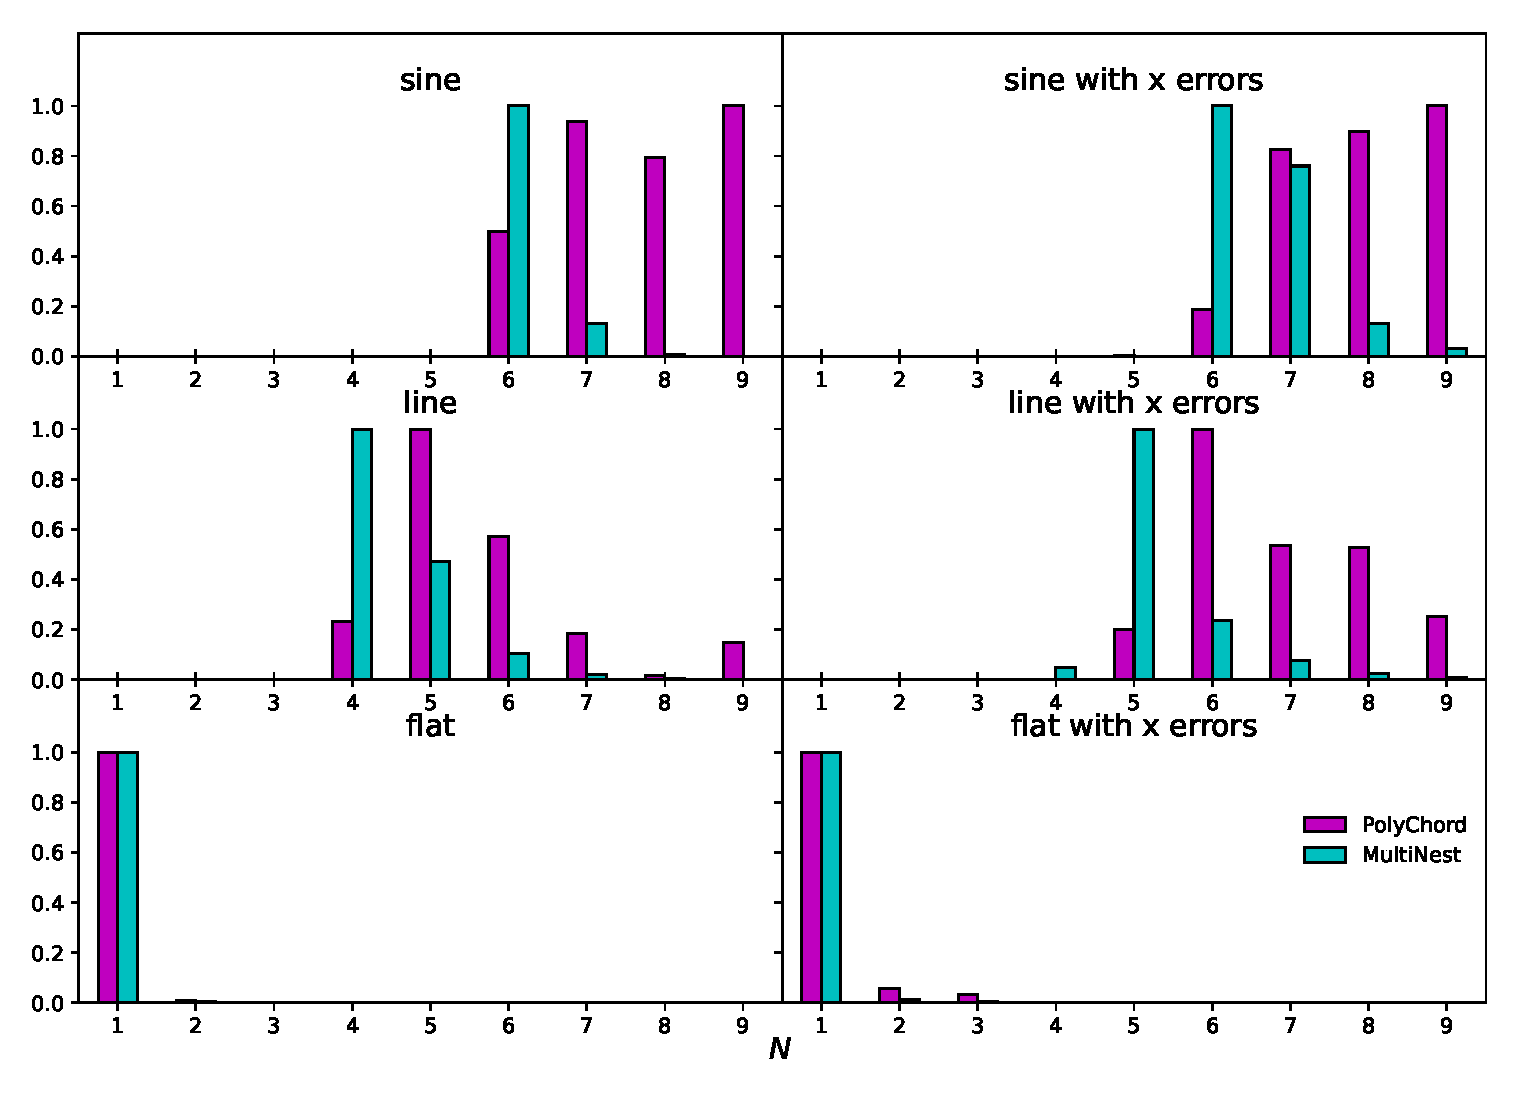
\includegraphics[width=14cm]{toysineN.eps}
  \caption{Histogram of posterior samples for adaptive \textit{linf}, for sine, line and flat cases, using either \texttt{PolyChord} or \texttt{MultiNest}. Left: $y$ errors only. Right: both $x$ and $y$ errors.}
  \label{fig:toysineN}
\end{figure}

The posterior distribution of $N$ for \texttt{AdaptiveLinf} are shown in figure \ref{fig:toysineN}, and their respective functional posterior plots in figure \ref{fig:toysineadaptive}. As expected, the flat case favours $N=1$. However, the line case doesn't favour $N=4$, instead preferring five or six nodes without and with $x$ errors respectively. Substituting the nested sampler \texttt{MultiNest} recovers $N=4$ at least in the $y$ errors only case; the posterior of $N$ is also shown in figure \ref{fig:toysineN}. However, \texttt{MultiNest} also favours 6 nodes for the sine wave, when one would expect the maximum number of nodes to be favoured. I am investigating this further. 

\begin{figure}[H]
  \centering
  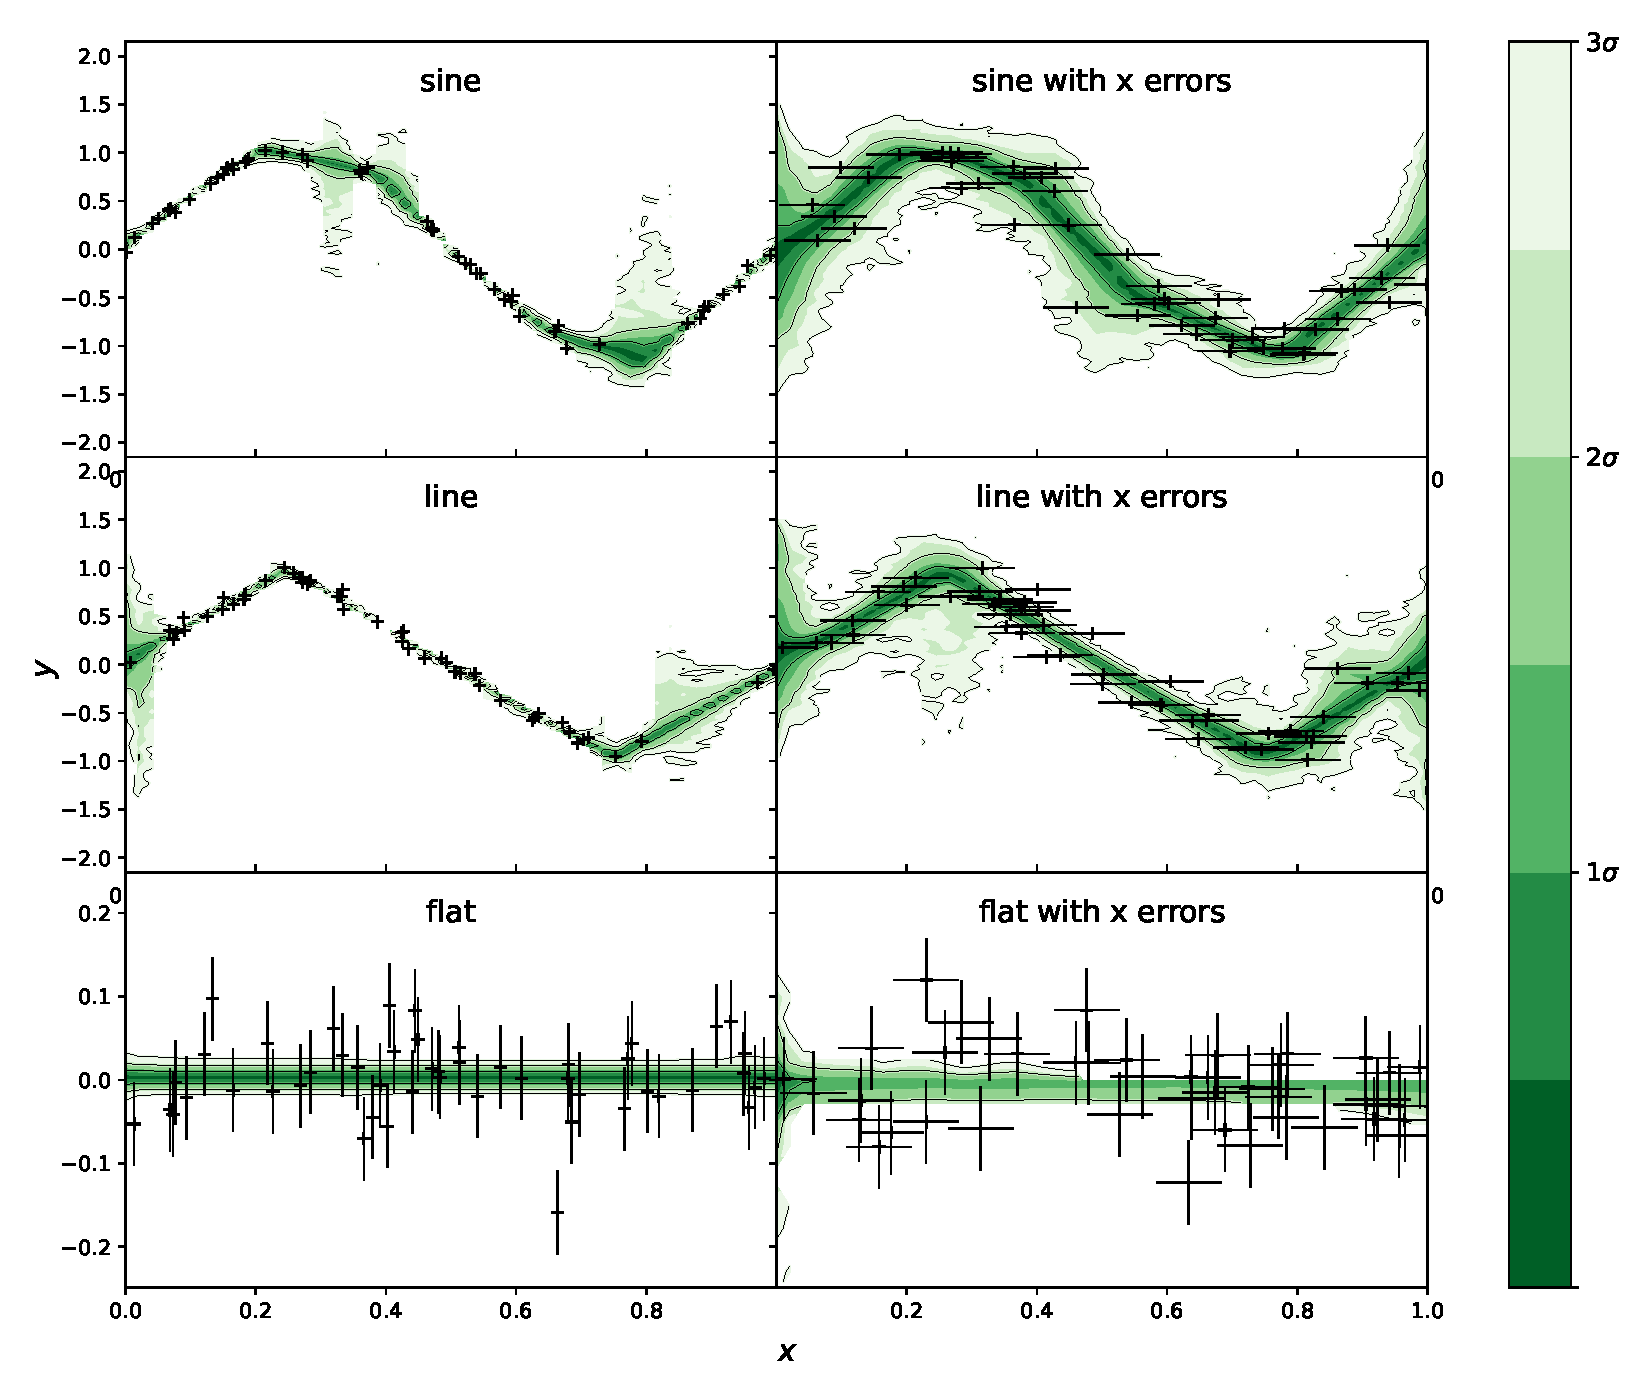
\includegraphics[width=16cm]{toysineadaptive.eps}
  \caption{Functional posterior contour plots of adaptive \textit{linf} posterior samples for sine, line and flat cases using \texttt{PolyChord}. Left: $y$ errors only. Right: both $x$ and $y$ errors. Note the different scale for the line case.}
  \label{fig:toysineadaptive}
\end{figure}

\newpage
\newpage

\section{Cosmological Applications}
\subsection{Cosmological codes}

\subsubsection{Cobaya}
\texttt{Cobaya} (\textbf{Co}de for \textbf{bay}esian \textbf{a}nalysis) is a sampling and modelling framework, intended for use with cosmology \cite{Cobaya}. It is written in Python, and provides interfaces to work with popular cosmological models \texttt{CAMB} and CLASS, the Planck likelihoods, and can sample using either a built-in MCMC algorithm, or the nested sampler \texttt{PolyChord}. \texttt{Cobaya} takes its input from a \texttt{.yaml} file, which specifies which models and likelihoods to use, and the priors for each of the parameters. 

\subsubsection{CAMB}
\texttt{CAMB} (Code for Anisotropies in the Microwave Background) is the Cosmological Boltzmann code I have used exclusively so far \cite{CAMB_1, CAMB_2}. It is one of two Boltzmann codes to which \texttt{Cobaya} can interface, the other is \texttt{CLASS} (Cosmic Linear Anisotropy Solving System, often labelled ``\texttt{classy}" to distinguish it from the class keyword). These codes calculate the theoretical CMB power spectrum for a given set of cosmological parameters, such as the Hubble constant $H_0$, primordial matter power spectrum $\mathcal P_\mathcal R(k)$, and the dark energy equation of state parameter $w$. I chose \texttt{CAMB} over \texttt{CLASS} as \texttt{CAMB} was used in the works I have been replicating, and currently \texttt{CAMB} is faster than \texttt{CLASS}, though this is subject to change as each of the codes continues to be updated.

\texttt{CAMB} is written in object-oriented FORTRAN90 and interfaced via Python, which allows \texttt{CAMB} to be used interactively with the speed of compiled code. It can be parallelised using \texttt{OpenMP} (Open Multi-Processing), with almost linear scaling up to 16 processes \cite{camb_mp}. 

\subsection{Primordial matter power spectrum}
To check that I am using \texttt{Cobaya} and \texttt{CAMB} correctly, I repeated the work in \cite{Handley2019}, where the primordial matter power spectrum is reconstructed using a linear spline. This is why I created my \textit{linf} package, as I can reuse it here.

The primordial matter power spectrum has the form:

\begin{equation}
  \mathcal P_\mathcal R(k) = A_s \left(\frac{k}{k_\textrm{pivot}} \right) ^ {n_s - 1},
\end{equation}
%
where $n_s$ is the scalar spectral index, and $A_s$ is the comoving curvature power at $k=k_\textrm{pivot}$ Then, taking logs of both sides, and converting to $\log_{10}{k}$ to match the literature and the original work \cite{Handley2019}, it can be seen that it is linear in log-log space, and therefore suitable for a linear spline reconstruction:

\begin{equation}
  \ln{\mathcal P_\mathcal R} = \ln{A_s} + \left(n_s - 1\right) \ln{\frac{k}{k_\textrm{pivot}}} = \ln{A_s} + \left(n_s - 1\right) \log_{10}{\frac{k}{k_\textrm{pivot}}} \ln{10}\textrm.
\end{equation}
%
$\mathcal P_\mathcal R(k)$ is of $\mathcal{O}\left(10^{-10}\right)$, but it is good practice in computation to work with parameters of $\mathcal{O}\left(1\right)$. Therefore, $\ln{\left(10^{10}\mathcal P_i\right)}$  was used as the $y$--parameter of the \textit{linf}. My code uses this scaling implicitly, i.e.\ \texttt{lnPi} refers to $\ln{\left(10^{10}\mathcal P_i\right)}$.

\begin{equation}
  \mathcal P_\mathcal R\left(\left\{\log_{10}{k_i}, \ln{\left(10^{10}\mathcal P_i\right)}\right\}\right) = 10^{-10} \exp{\left[{\textrm{linf}\left(\left\{\log_{10}{k_i}, \ln{\left(10^{10}\mathcal P_i\right)}\right\}\right)}\right]}\textrm.
\end{equation}
%
Unlike the toy example where I was working with \texttt{PolyChord} directly, \texttt{Cobaya} understands each of the model parameters separately. Also, what \texttt{PolyChord} calls a ``prior" is the inverse cumulative distribution function of the prior, while \texttt{Cobaya} understands priors more literally. Applying this inverse to points uniformly distributed in the unit hypercube $[0, 1]^D$ returns points distributed according the the prior. Therefore, the interleaved uniform/sorted-uniform prior in my \texttt{linf} package cannot be used here. Instead, each of the $\log_{10}{k_i}$ parameters is given its own uniform prior, with the sorted constraint implemented in a separate prior, e.g:
\begin{verbatim}
  lambda lgk1, lgk2, lgk3, lgk4, lgk5, lgk6, lgk7: np.log(lgk1 < lgk2 < lgk3 < lgk4 
    < lgk5 < lgk6 < lgk7)
\end{verbatim}
for nine total nodes, where $\lg$ is shorthand for $\log_{10}$. This, along with including the parameters in the parameter block, made for laborious typing (even with Python's compact comparison operator chaining), so I automated writing the yaml files with a Python script.

The likelihoods used in the toy examples of section \ref{toyexamples} are similarly also not suitable for use by \texttt{Cobaya}, plus the highly non--trivial task of turning the CMB measurements from Planck into a likelihood function for dark energy. Fortunately \texttt{Cobaya} interfaces with official clik code, which calculates these likelihoods. \cite{planck_likelihoods_1, planck_likelihoods_2}. I used the following likelihoods: lensing, low--$l$ $EE$ and $TT$, high--$l$ $TTTEEE$ and Sunyaev–Zeldovich (SZ). \texttt{Cobaya} takes care of the installation of the codes, which just need to be mentioned in the likelihood block of the input yaml file.

\texttt{Cobaya} has a built-in option for the user to provide their own $\mathcal P_\mathcal R(k)$. This is done by specifying \texttt{external\_priomoridal\_pk:} \texttt{True} in the \texttt{CAMB} block, and providing the path to a class which will provide $\mathcal P_\mathcal R(k)$. This class must inherit from \texttt{cobaya.Theory}, needs a \texttt{calculate} method which adds the $k$ and $\mathcal P_\mathcal R(k)$ values to the state dictionary, and a \texttt{get\_primordial\_scalar\_pk} method which returns this part of the state. The class variable \texttt{params} specifies the parameters required for the calculation. \texttt{CAMB} then internally uses a cubic spline between these values.

I expressed my ten different \texttt{Theory}s (nine vanilla plus adaptive) using inheritance. The \texttt{LinfPk} inherits from \texttt{Theory}, and defines the \texttt{calculate} and \texttt{get\_primordial\_scalar\_pk} methods. \texttt{calculate} depends on \texttt{self.linf}, which is specified in its child classes \texttt{VanillaPk} and \texttt{AdaptivePk}. \texttt{AdaptivePk} is complete as it specifies its own \texttt{params}, while \texttt{Vanilla[1-9]} specify them for  \texttt{VanillaPk} for the nine vanilla cases. A class diagram is shown in figure \ref{fig:PkUMLDiagram}. The functional posteriors from the vanilla cases are shown in figure \ref{fig:Pk_vanilla_100}, using 100 \texttt{PolyChord} live points. Their respective evidences are shown in figure \ref{fig:PklogZ}, along with the corresponding values for the adaptive case, split by $N$. The two sets are clearly different, in particular the most unlikely cases of $N=1$ and $N=9$. For the adaptive case, these each have an effective sample size of approximately one. This is because PolyChord has successfully identified them as low evidence modes, and has saved computation time by not sampling them in more detail.

\begin{figure}
  \centering
  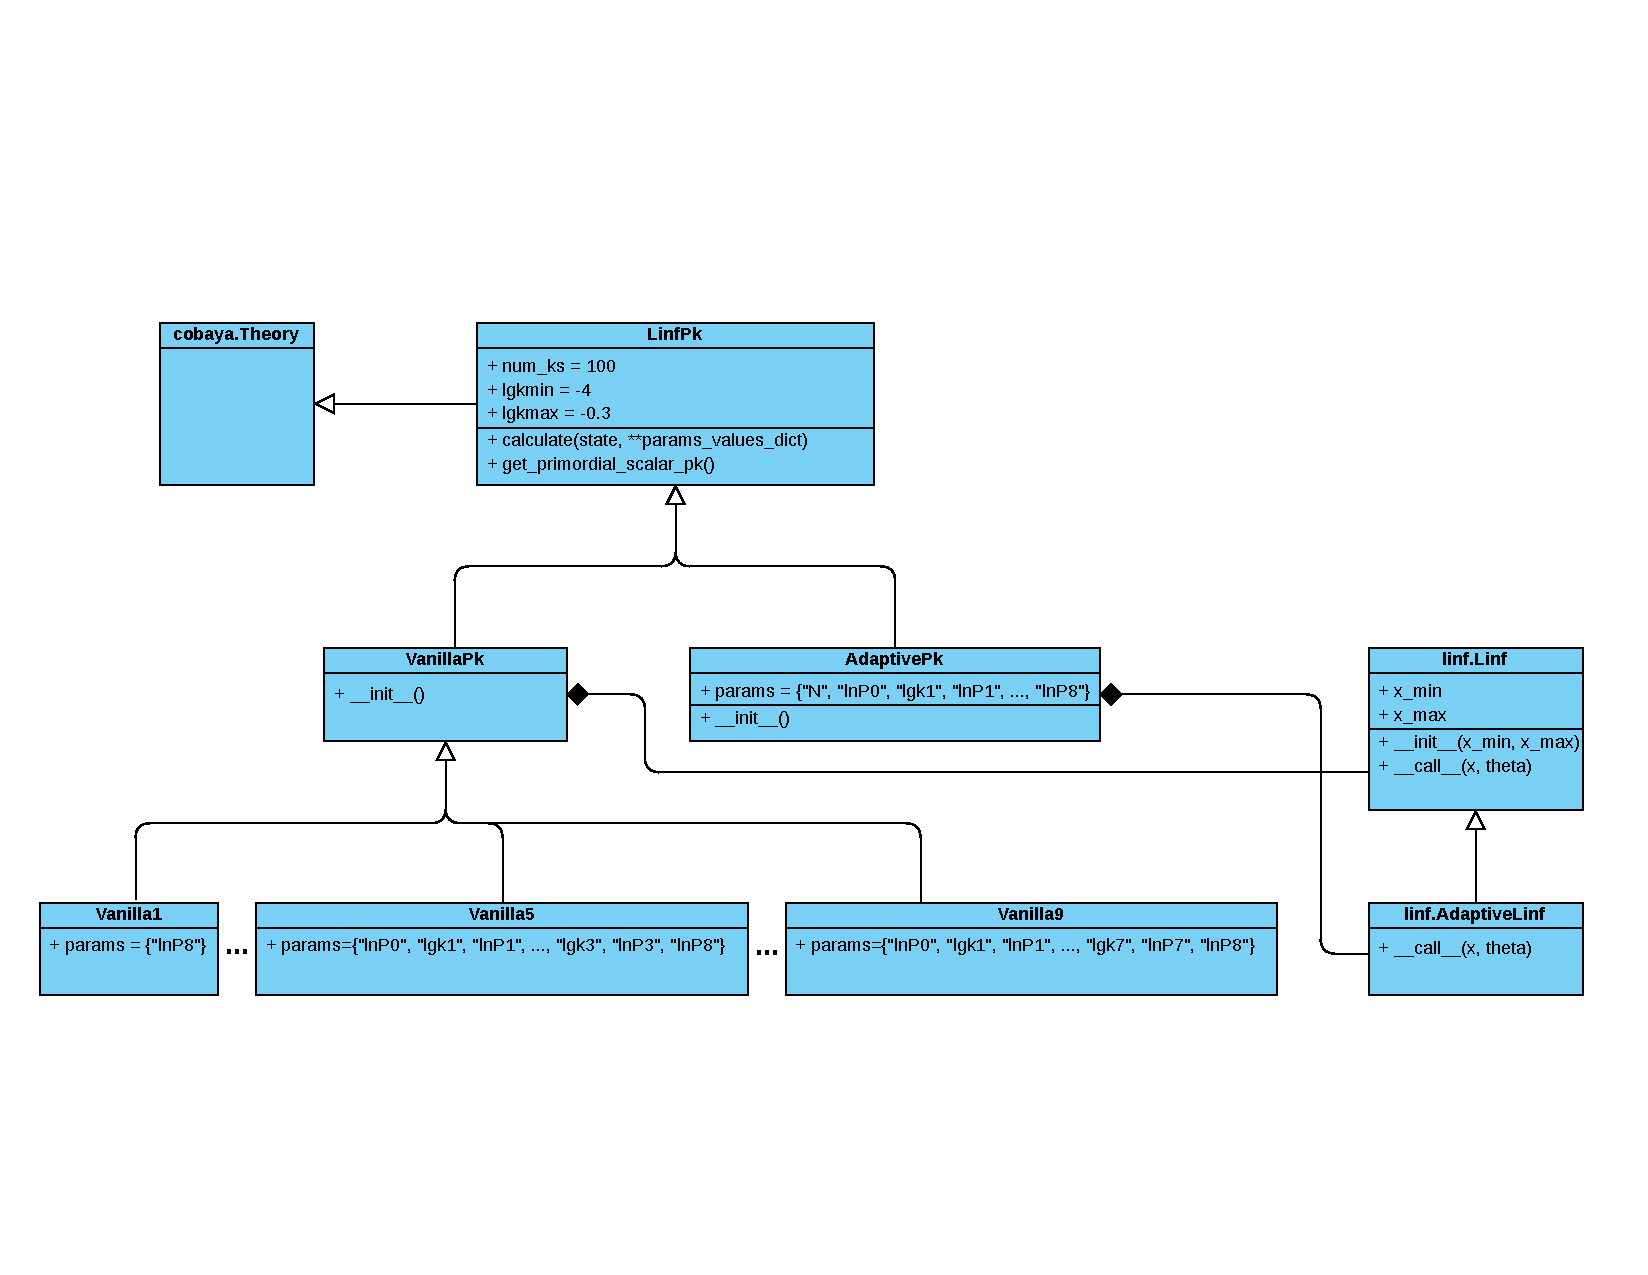
\includegraphics[width=16cm]{Pk_linf.pdf}
  \caption{Class diagram for the Theory subclasses used to reconstruct the primordial matter power spectrum with a linear spline. \texttt{LinfPk} defines the \texttt{calculate} and \texttt{get\_primordial\_scalar\_pk} methods, then the constructors for \texttt{VanillaPk} and \texttt{AdaptivePk} specifies which type of \texttt{linf} to use. \texttt{AdaptivePk} also specifies its \texttt{params} class attribute, while for the nine vanilla cases this is specified by the children of \texttt{VanillaPk}.}
  \label{fig:PkUMLDiagram}
\end{figure}

\newpage

\begin{figure}[H]
  \centering
  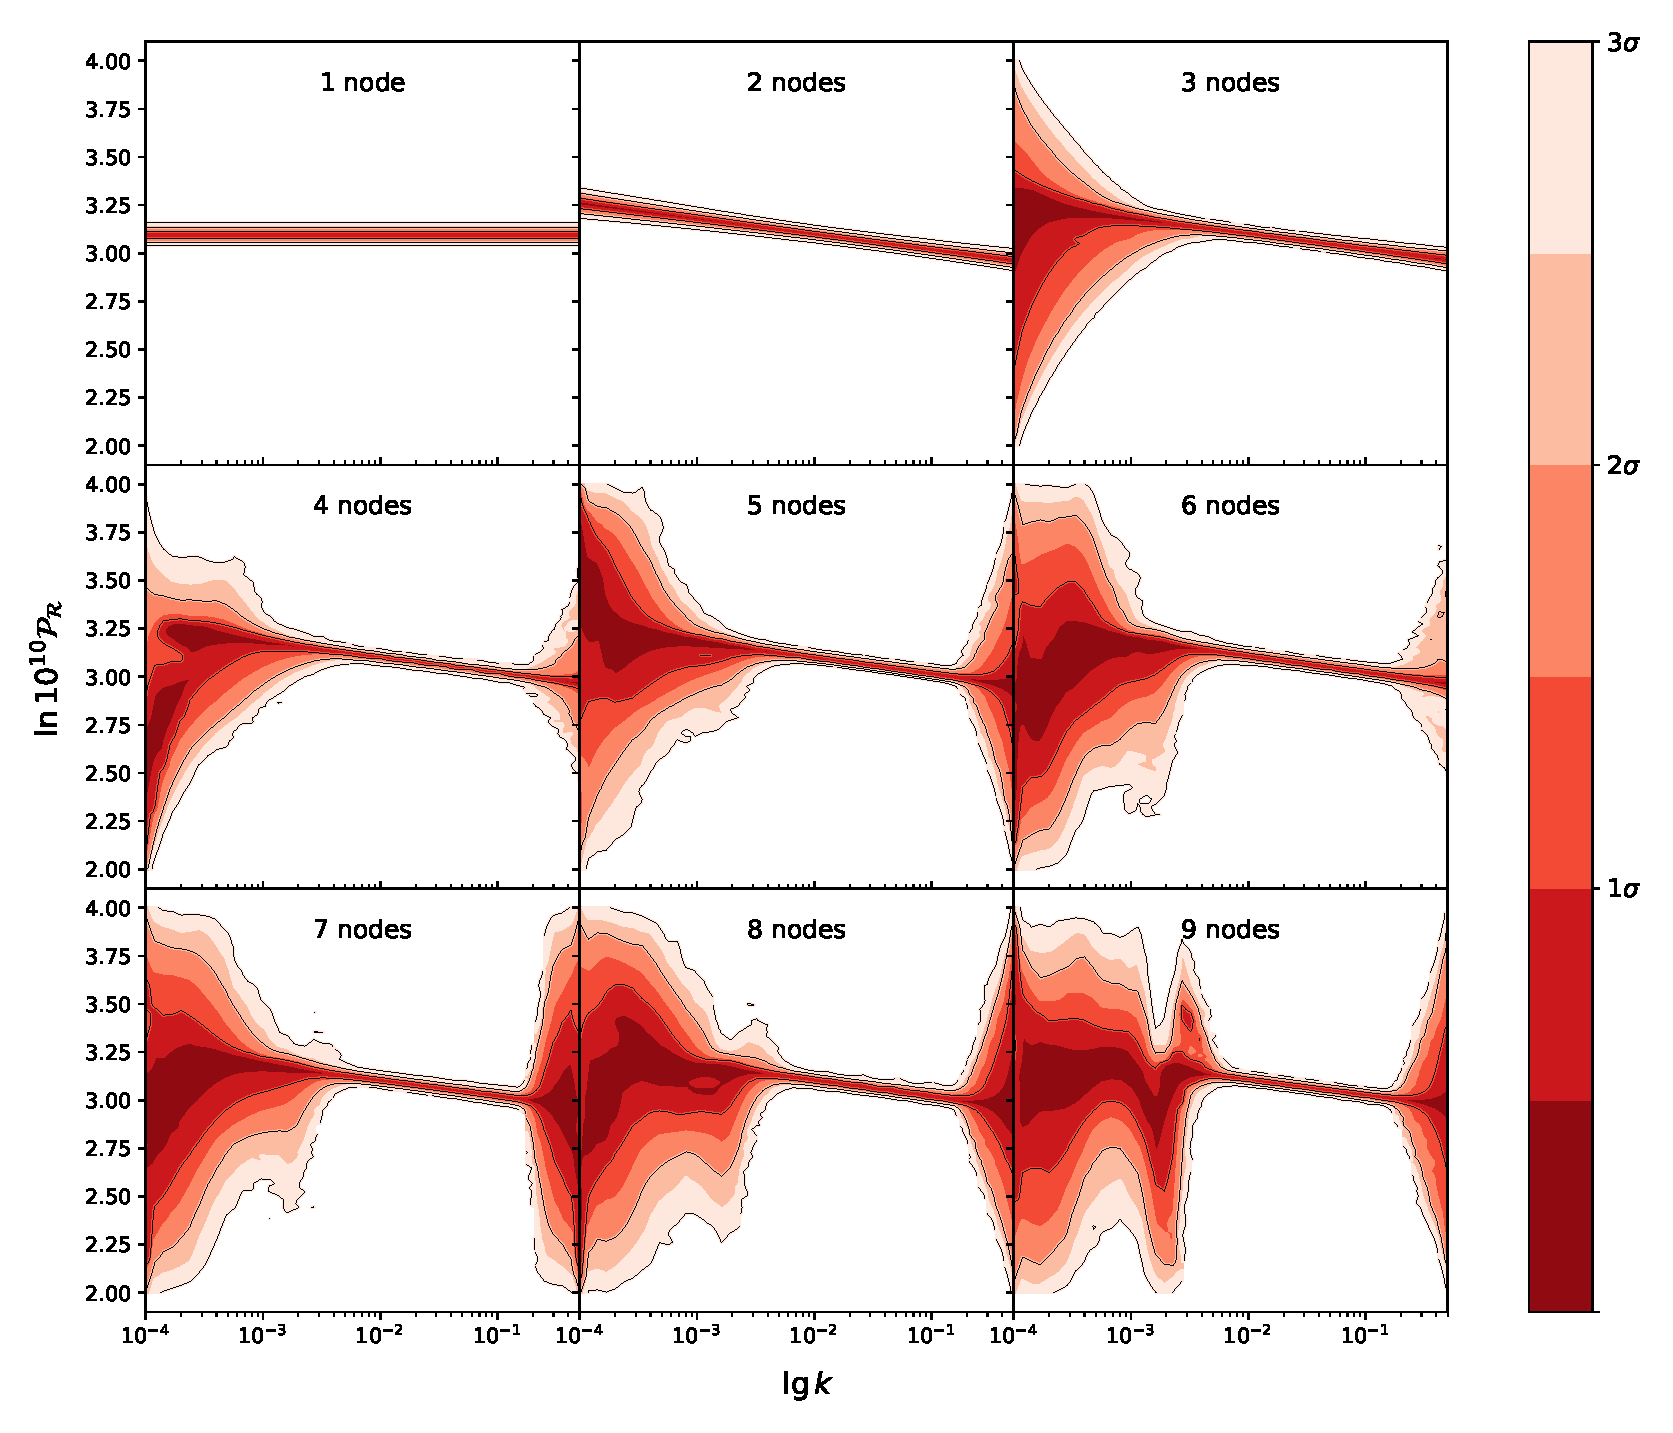
\includegraphics[width=16cm]{vanilla100.eps}
  \caption{Functional posterior contour plots for the \textit{linf} reconstruction of the primodial matter power spectrum, with fixed numbers of nodes from 1 to 9. 100 live points was used for each of these runs.}
  \label{fig:Pk_vanilla_100}
\end{figure}

\newpage

\begin{figure}[H]
  \centering
  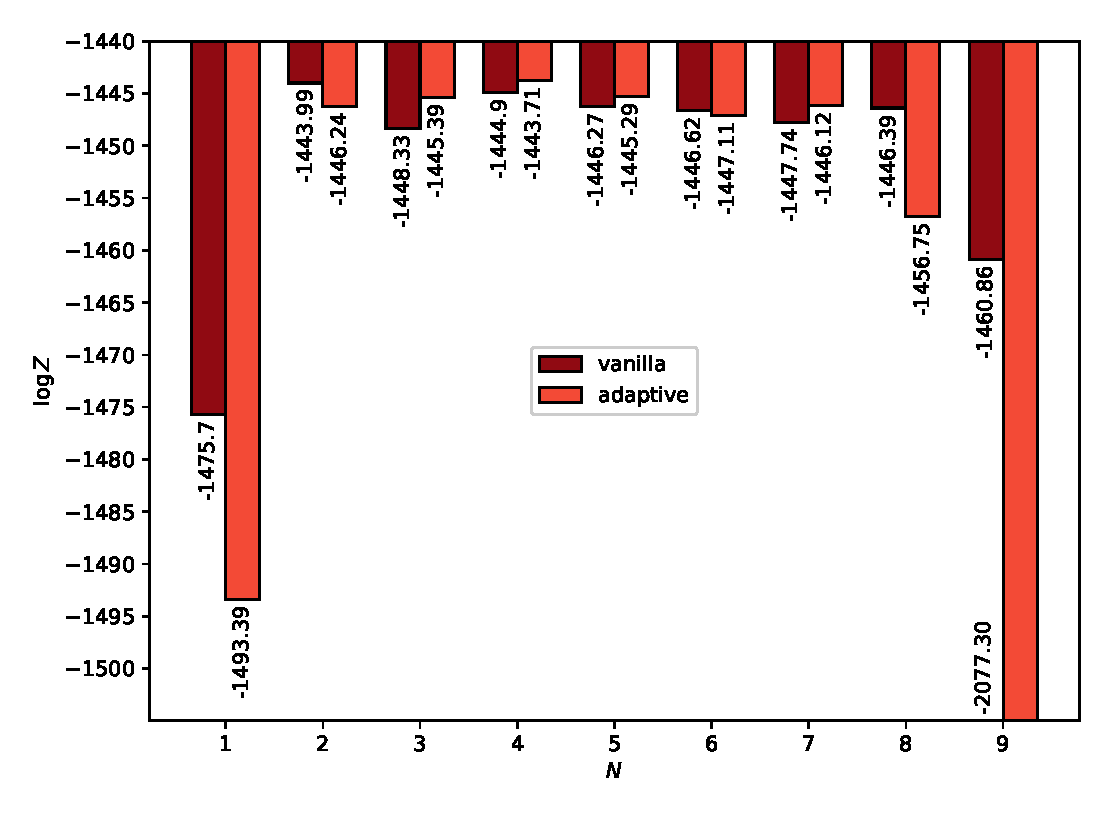
\includegraphics[width=13cm]{PklogZ.eps}
  \caption{Evidence values for the primordial matter power spectrum for each of the vanilla reconstructions shown in figure \ref{fig:Pk_vanilla_100}, and the adaptive reconstructions, split by $N$ value to calculate $\log{Z}$ for each.}
  \label{fig:PklogZ}
\end{figure}

\subsection{Dark energy}
\label{sec:de}

All the exercise with toy sine models and the primordial matter power spectrum was building up to investigate the dark energy equation of state. The equation of state of a perfect fluid is characterised the ratio of its pressure to its density: $w = p/\rho$. The goal is to perform a similar spline ``\textit{linf}" reconstruction to $\mathcal P_\mathcal R(k)$ with $w(a)$.

Since dark energy exists as an explanation for the cosmological constant, i.e.\ a fluid with $w=-1$, this needs to be reflected in the prior and \texttt{AdaptiveLinf}. Therefore, I modified my \texttt{AdaptiveLinf} so that for $N=0$ (or more accurately, $0\le N <1$) it is constant at -1. This is more appropriate than the cosmological constant being only the $w_{N_\textrm{max}-1} = 1$, $1\le N<2$ element of the entire prior volume.

The primordial matter power spectrum is unique in \texttt{Cobaya} in having the \texttt{external\_primordial\_pk} option. The primordial power spectrum is separate from the rest of the parameters passed to \texttt{CAMB}, which are either used to compute the transfer functions or specify non--linear behaviour. The transfer functions are then applied to the power spectrum to compute the spectra we see today. This means that the primordial power spectrum can be changed without needing to recompute the transfer functions, so can be sampled independently.

Changing dark energy is less straightforward as \texttt{Cobaya} only supports the cosmological constant with \\ $w=-1$, $w =$ constant with some other value, or $w(a) = w+(1-a)w_a$. \texttt{CAMB} includes a \texttt{set\_dark\_energy\_w\_a()} method to supply a table of $w$ values. My goal was then to echo the primordial power spectrum functionality with a \texttt{external\_wa} option, which takes values of $w$ and $a$ from a \texttt{cobaya.Theory} with a \texttt{get\_dark\_energy()} method, and provides these to \texttt{CAMB}. Like $\mathcal P_\mathcal R(k)$, \texttt{CAMB} internally performs a cubic interpolation between these values.

\texttt{CAMB} suffers segmentation faults if the $w(a)$ table starts at $a=0$. The workaround suggested by the developers was to start at a low value of $a$, they suggested $10_{-10}$. It also only accepted float values for $a$ and $w$, using $a=1, w=-1$ would also cause a fault. Therefore, I added a validation step to the \texttt{CAMB} Python interface which checks that the array of $a$ are all greater than zero, and casts them to float. This is now part of the \href{https://github.com/cmbant/CAMB}{master branch of \texttt{CAMB}}\footnote{\href{https://github.com/cmbant/CAMB}{https://github.com/cmbant/CAMB}}.

I chose a prior of $a_i$ sorted-uniform in $[0.1, 1]$, and $w_i$ uniform in $[-2, -0.01]$. As this range extends below $-1$, termed ``Phantom energy", this requires using the Parameterised Post-Friedmann dark energy, as a model with a single scalar field cannot cross $w=-1$ \cite{PPF}. 

The challenging part here was to understand the correct place in the \texttt{Cobaya} code to add this change. As $w(a)$ needs to be set with the other \texttt{CAMB} transfer function parameters, I could not copy the existing code for $\mathcal P_\mathcal R(k)$. Instead, I ran \texttt{Cobaya} in debug mode with $w=\textrm{const.}$ to find where it provides this value to \texttt{CAMB}. Once I found it (\texttt{cobaya.theories.camb.camb.CAMB.set()}), I appended a check for \texttt{external\_wa}, and if so then pass the values of $w$ and $a$ to the instance of \texttt{CAMBparams}, the object which stores the parameters for \texttt{CAMB}. This didn't work, which manifested itself as either segmentation faults or getting very different results with a flat \textit{linf} ($N=0$) when compared to varying $w$ directly. This is because the order in which parameters are provided to \texttt{CAMB} is important. Dark energy should be set \textbf{first}, as when \texttt{CAMB} is provided with \texttt{theta\_MC\_100} ($100 \times$ the ratio of the sound horizon to the angular diameter distance), it then uses dark energy to calculate $H_0$. It is more efficient to sample \texttt{theta\_MC\_100} than $H_0$ as it is less correlated with other parameters \cite{CosmoMCReadMe}. Therefore, I changed \texttt{set()} so it creates a fresh instance of \texttt{CAMBparams}, sets the table of $w$ and $a$, then sets the the rest of the cosmology so that $H_0$ is computed correctly.

To avoid any issues arising from using the internal cubic spline (which the \texttt{CAMB} documentation notes is quite slow \cite{CAMBdocs}), I created several branches of \texttt{Cobaya} in parallel. \textit{external\_wa} matches the description above, \textit{flat\_wa} takes the last value from the \textit{linf} and sets $w$ directly, and \textit{linear\_wa} takes the first and last values from the \textit{linf}, uses these to calculate $w$ and $w_a$, and sets those. I compared the \textit{flat\_wa} branch against the Planck 2018 MCMC chains, and \textit{linear\_wa} against an unmodified \texttt{Cobaya} allowing $w_a$ to vary, with present day $w=-1$. Only once I was convinced these were consistent did I then use the full \textit{external\_wa} version.

At the start of each run, \texttt{Cobaya} times each of the theories, and works out the appropriate oversampling factor for each of them. At the moment, I have been manually specifying in the input yaml file for \texttt{Cobaya} that the dark energy parameters should be sampled with the rest of the cosmological parameters, rather than separately, as I have found this roughly halves the runtime. I would like to automate this, as doing this manually requires the user to also specify the oversampling factors.

Due to the large computational cost associated with performing each run, and the known issues with \texttt{PolyChord} clustering, I have only produced low resolution runs so far. I used 80 live points rather than the 100 for the primordial power spectrum, since this could reliably finish within a single 12 hour run for \textit{flat\_wa} and \textit{linear\_wa}. I am also finding that, when \texttt{anesthetic} reads the \texttt{PolyChord} chains, a few ($\mathcal{O}(1\%)$) of the samples have NaN weight and loglikelihood. This can be worked around by simply dropping those rows and recalculating, but it is important I understand why this is happening. 

I have included some provisional posterior plots in figure \ref{fig:externalwa}, for $N_\textrm{max}$ = 1, 2, 3, 4 and 9. The posterior distributions of $N$ are shown in figure \ref{fig:darkN}. To also save running time while working and testing, I continued to only use the Planck 2018 likelihoods that I used with the primordial matter power spectrum. However, these do not provide a tight bound for dark energy, with $w=-1.57_{-0.40}^{+0.50}$ from Planck's own analysis. \cite{planck_6}. This makes sense, the CMB is from the early universe, and therefore not strongly coupled to the late--time acceleration of the universe's expansion due to dark energy. Functional posteriors are shown in figure \ref{fig:externalwa}. In S.~Hee's work, they also use the Baryonic Acoustic Oscillation (BAO) and IA supernovae likelihoods, which both provide measurements of the Hubble parameter, which is strongly dependent on dark energy \cite{Sonke, BAO1, BAO2, BAO3, SNIa}. The functional posterior including these likelihoods for $N_\textrm{max}=9$ is shown in figure \ref{fig:darkNbao}, and the $N$ posterior is also shown in the sixth box of figure \ref{fig:darkN}. Here the cosmological constant ($N=0$, $w=-1$) case dominates. I will not draw any definitive conclusions until the clustering issues with \texttt{PolyChord} have been solved, so that I can rerun this with higher resolution.

\newpage

\begin{figure}[H]
  \centering
  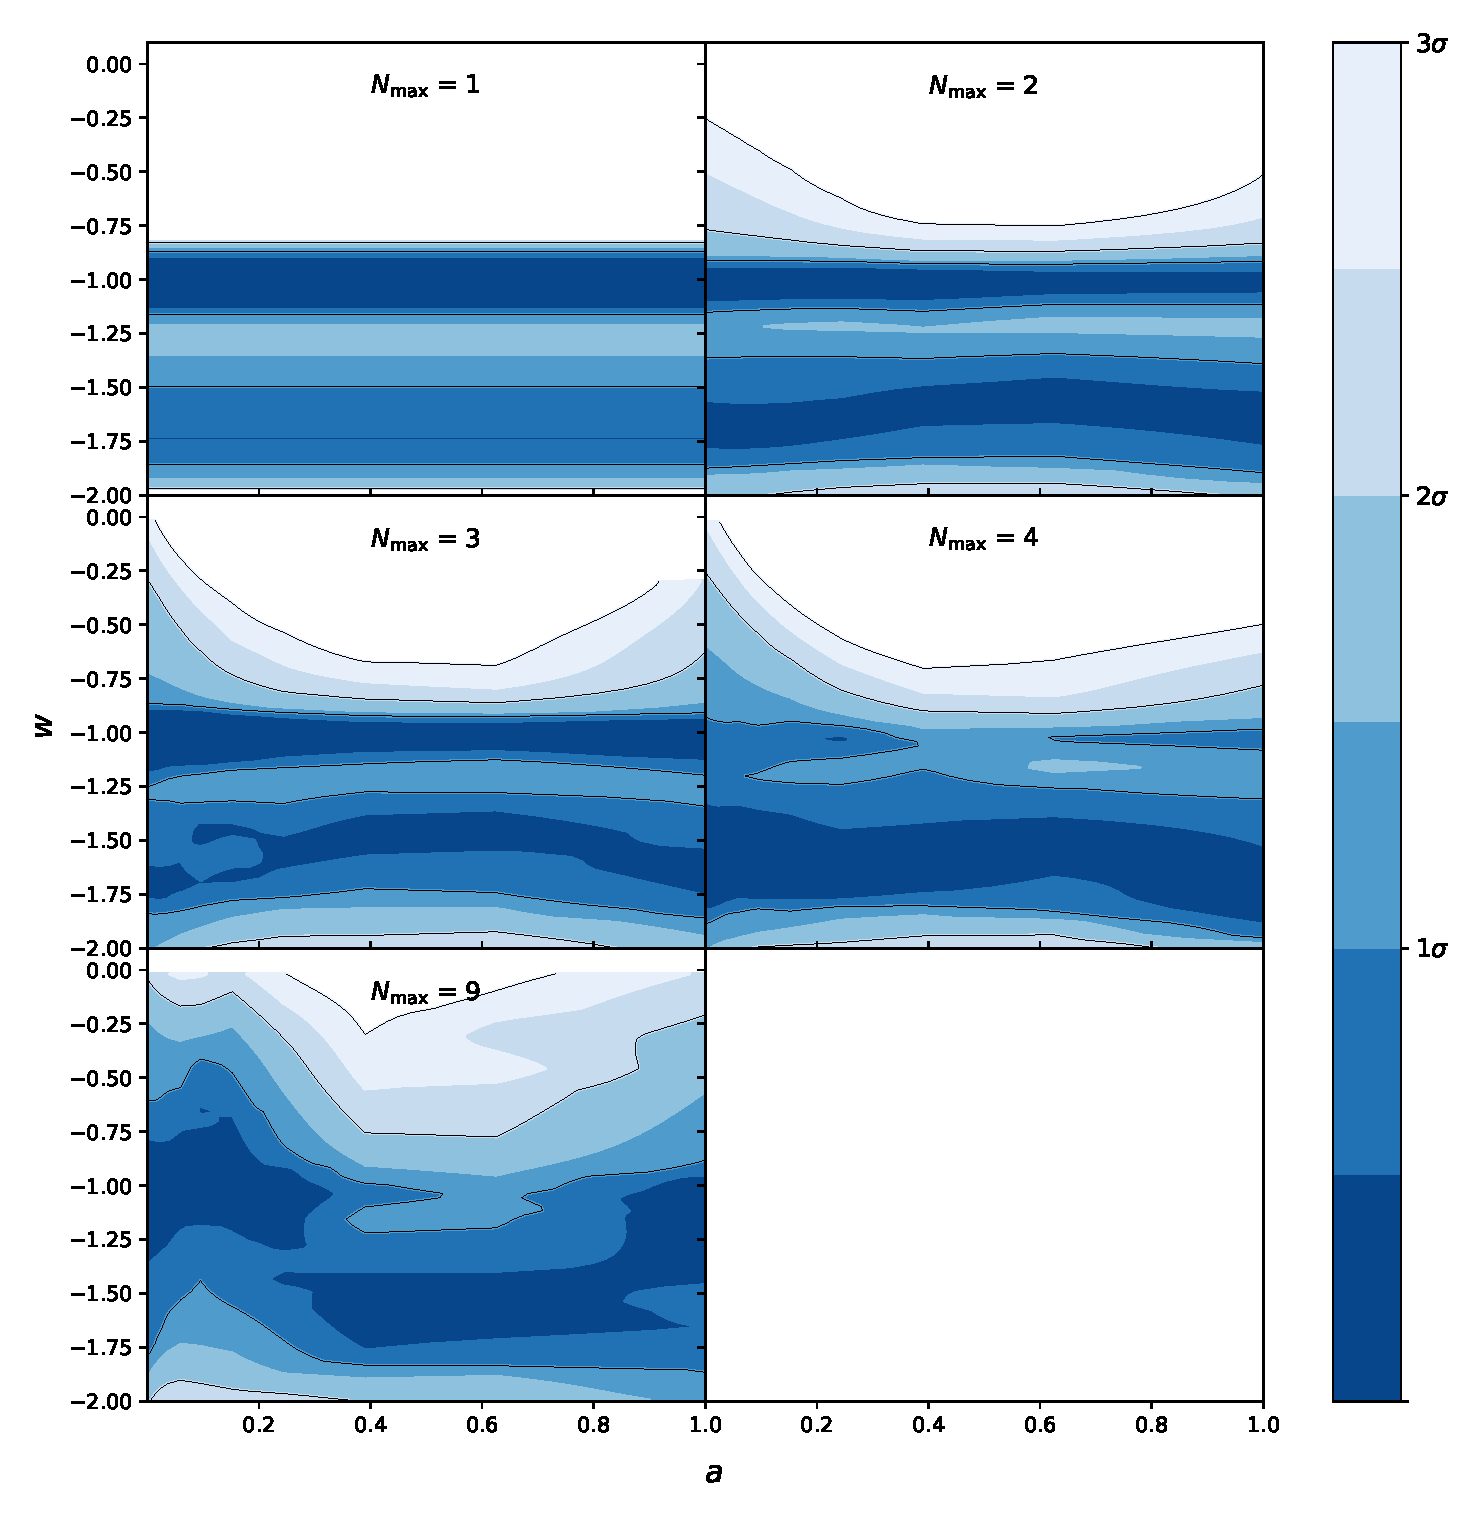
\includegraphics[width=16cm]{adaptivew.eps}
  \caption{Posterior plots using an \texttt{AdaptiveLinf} as a model for the dark energy equation of state parameter, with different values of $N_\textrm{max}$. These use the Planck 2018 likelihoods only. For $N_\textrm{max}\le 3$, $w=-1$ is still a dominant mode, as $N_\textrm{max}$ increases further, values around -1.7 to -1.5 begin to appear. This is in line with $w=-1.57_{-0.40}^{+0.50}$ calculated by Planck 2018 \cite{planck_6}.}
  \label{fig:externalwa}
\end{figure}

\newpage

\begin{figure}[H]
  \centering
  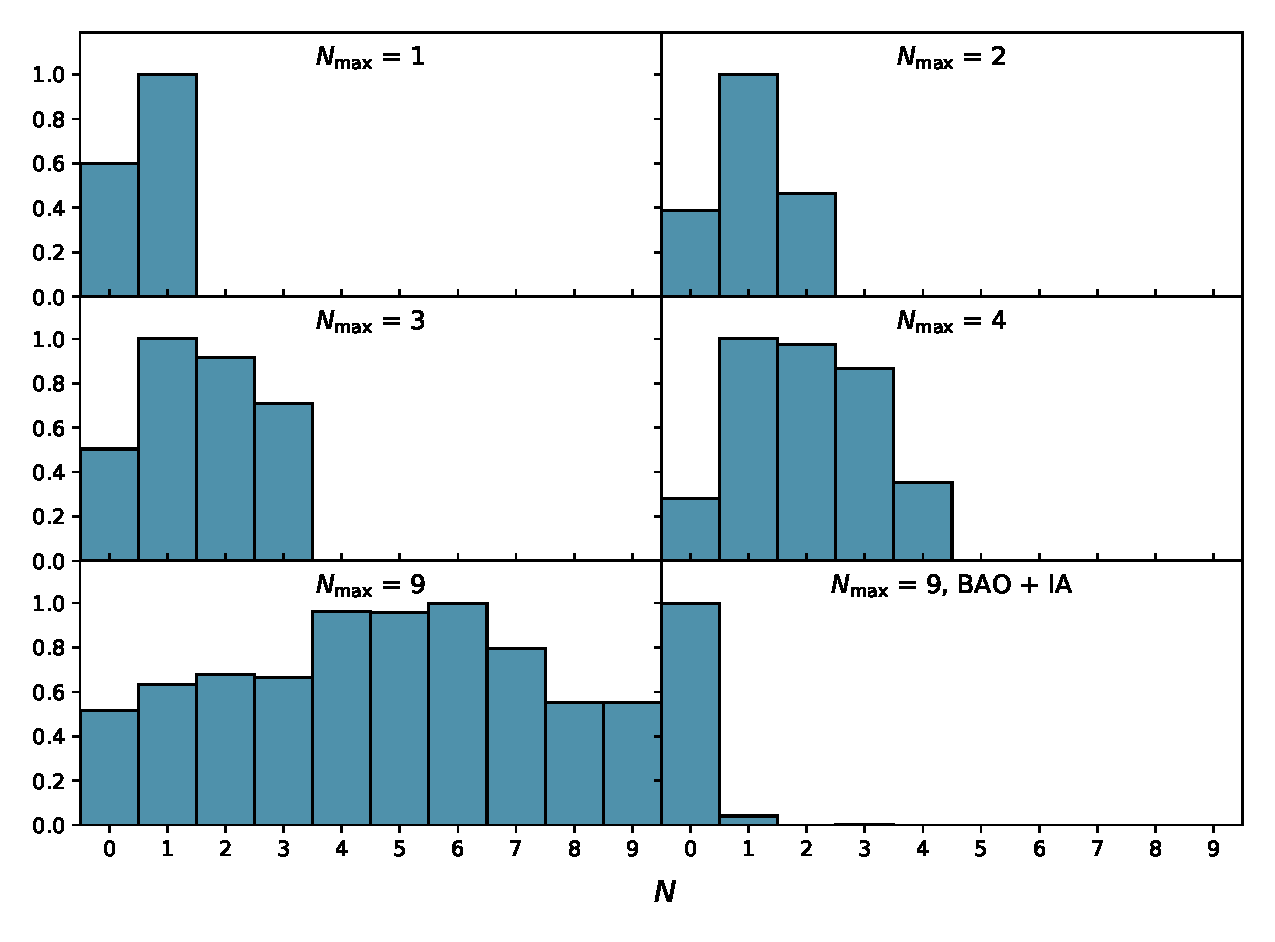
\includegraphics[width=13cm]{darkN.eps}
  \caption{Histograms of posterior samples of the number of nodes of an \texttt{AdaptiveLinf} used to reconstruct the dark energy equation of state parameter. $N=0$ corresponds to $w=-1$, the cosmological constant. The first five cases use different maximum $N$, and do not favour the cosmological constant. Adding in Baryonic Acoustic Oscillations and IA supernovae data recovers the cosmological constant in the sixth plot.}
  \label{fig:darkN}
\end{figure}

\begin{figure}[H]
  \centering
  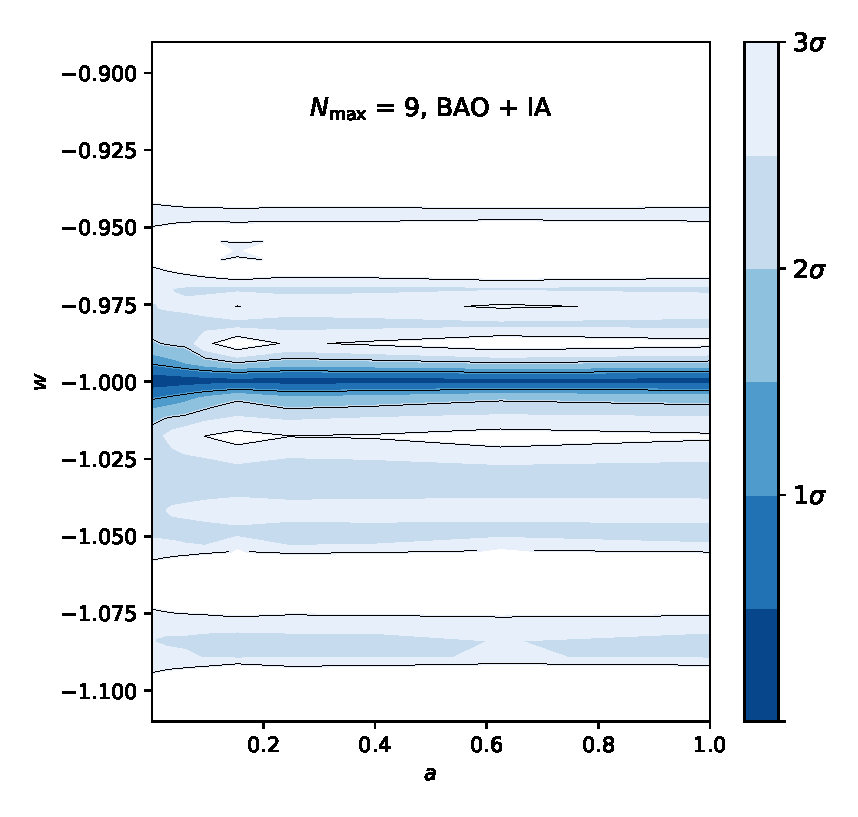
\includegraphics[width=9cm]{darkNbao.eps}
  \caption{Posterior plots using an \texttt{AdaptiveLinf} as a model for the dark energy equation of state parameter, using the Baryonic Acoustic Oscillations and IA supernovae data in addition to the Planck likelihoods. This recovers the cosmological constant $w=-1$.}
  \label{fig:darkNbao}
\end{figure}

\newpage

\section{PolyChord Revisited: Clustering}
\label{sec:polychord_revisited}

To produce results more quickly I used 100 \texttt{PolyChord} live points, intending to increase this to 25 $\times$ number of dimensions $= 25 N_\textrm{dims} \approx800$ for the final run to put in this report, as advised \cite{PolyChord_1, PolyChord_2, Sonke}. However, for the three-node case this causes a problem. $\mathcal P_\mathcal R(k)$ is most tightly constrained to a linear slope for $k = 10^{-2.5} - 10^{-0.8}$, and much less so outside of this. Two high-likelihood modes are expected, one with a node to the left of this range, and one to the right. The posterior plot of the \textit{linf} should therefore consist of a narrow centre section, with the less constrained parts fanning out at either side from each of the modes. This is what is seen with 100 live points. However, when the resolution is turned up to $25N\textrm{dims}=725$, only the left hand mode is present. We believe this to be because the greater density of live points means the parameter space gap between the two modes is bridged, so \texttt{PolyChord} fails to identify them as two separate clusters, which is necessary for it to function properly. The posterior samples for the internal node for both resolutions and their respective functional posteriors are shown in figure \ref{fig:N3}

Since the original paper \cite{Handley2019}, improvements have been made to \texttt{CAMB}, in particular its ability to account for the non--linear lensing effects due to matter between the surface of last scattering and Earth. However, there is an issue with the \texttt{Cobaya} documentation with respect to how to turn off these non--linear effects, so I have been unable to test whether removing them recovers the right--hand mode. This is apparent as turning this off should increase \texttt{CAMB}'s speed and therefore its oversampling factor, which has not happened.

\begin{figure}[!ht]
  \centering
  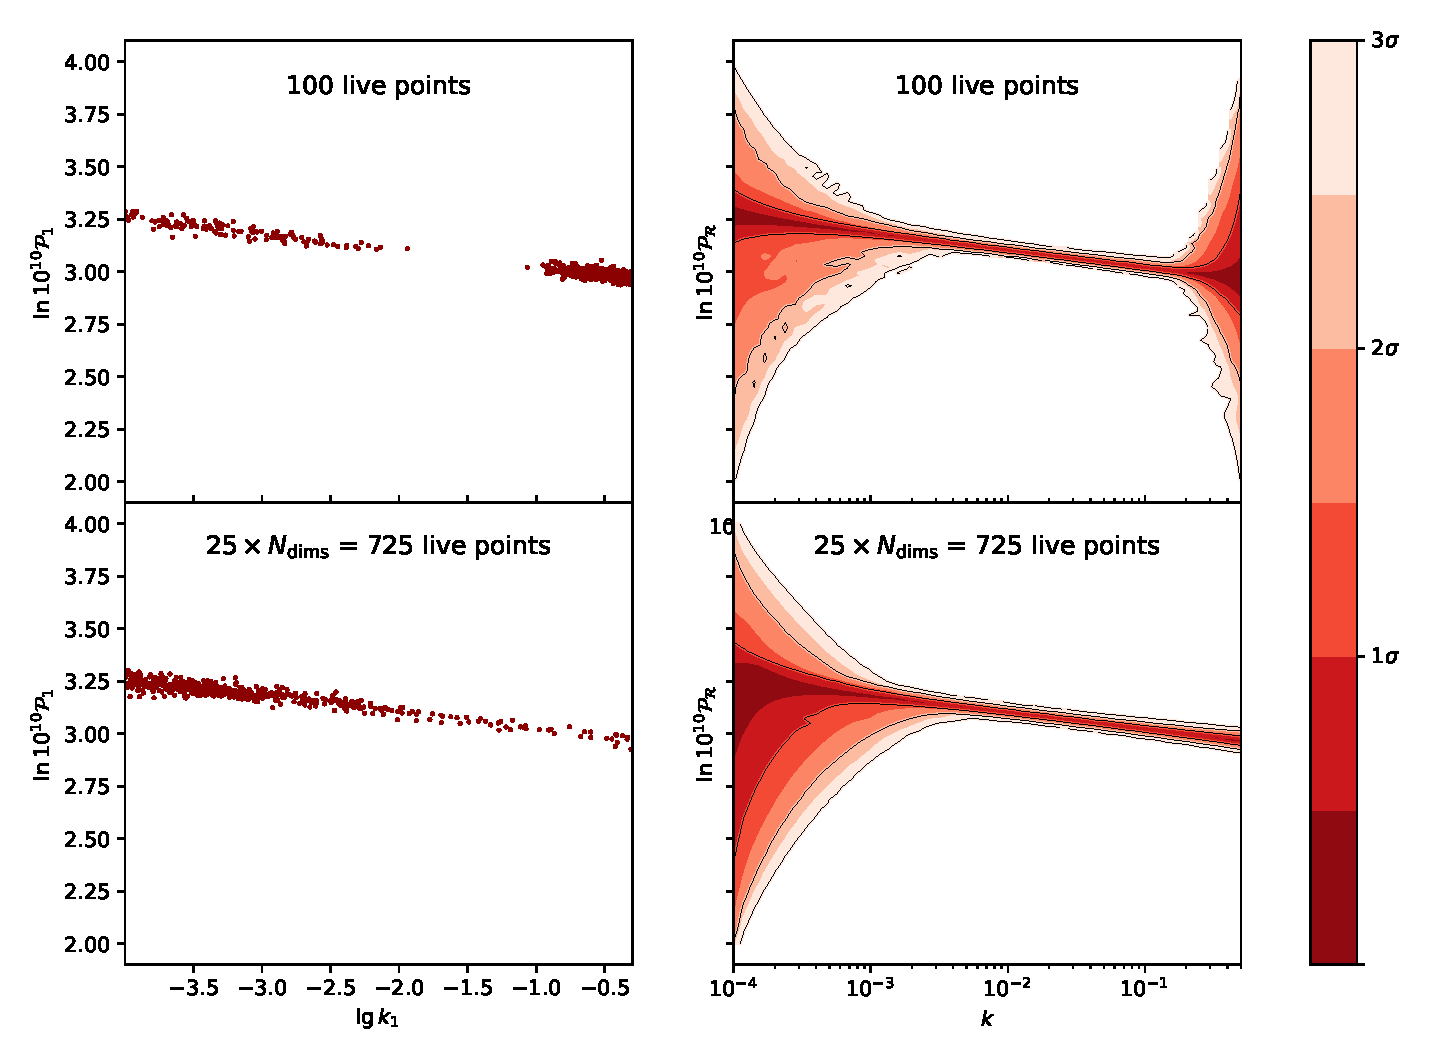
\includegraphics[width=15cm]{N3comparison.eps}
  \caption{Left: posterior samples of the internal node of three for the \textit{linf} primordial matter power spectrum. With 100 live points, there are two distinct modes, which \texttt{PolyChord} has identified as two separate clusters. Increasing the resolution to $25 \times N_\textrm{dims}$ causes the mode with the internal node at high $k$ to be lost. Right: posterior of the \textit{linf} function for the primordial matter power spectrum. The loss of the mode with the internal node at high $k$ means the distribution doesn't fan out on the right.}
  \label{fig:N3}
\end{figure}

\newpage

\subsection{Custom Clustering}
To investigate the clustering issue, Dr.~Handley and I have modified \texttt{PolyChord} to use a user-defined clustering algorithm. By default, \texttt{PolyChord} uses a recursive version of the K--nearest--neighbours (KNN) algorithm:
\begin{verbatim}
function K_nearest_neighbours(distance2_matrix[n_points, n_points]):
  K = min(10, nlive)
  calculate the K nearest neighbours for each point
  do n = 2 to K:
    if two points in either of each other's n nearest neighbours: 
      they are in the same cluster
    if cluster_list unchanged since n-1: return cluster_list
    if n == K: 
      K = min(2*K, nlive)
      recalculate K nearest neighbours for each point
    
  if number of clusters >= 2: search recursively
  return cluster_list
\end{verbatim}
Browsing though alternatives, K-means seems the most recommended and robust alternative \cite{MacKay2003}, and is included in the SciKit Learn Python package \cite{scikit-learn}. The K in both names is misleading as their meaning is unrelated, in KNN it refers to the number of neighbours to consider, in K-means K is number of clusters to consider.


\begin{verbatim}
function K_means(position_matrix[n_points, d_dimensions], K):
  # initialisation
  responsibilities = zeros[K, n_points]
  means = K random positions
  
  # assignment
  while means are changed since previous pass:
    distance2 = (x-means)^2
    for j = 1 to n:
       i_closest = 1
       
       for i = 2 to k:
         if distance2[i, j] < distance2[i, j]:
           responsibility[i_closest, j] = 0
           responsibility[i, j] = 1
           i_closest = 1
         elif d[i, j] == d[i_closest, j]:
           assign to whichever has lower responsibility
           
    for i = 1 to K:
      R = sum(responsitlities[i, :])
      if R > 0:
        means[i, :] = dot(responsibilities[i, n], x[n]) / R
\end{verbatim}
 
K-means is not guaranteed to find the optimal set of clusters; this can be helped by carefully choosing the intial guess for the means. K-means++ uses the following initialisation steps \cite{kmeans++}:
\begin{enumerate}
  \item Choose one of the data points as the first mean.
  \item Calculate the squared distance of each of the remaining points to the nearest point that has already been chosen.
  \item Choose another point, weighted inversely to these squared distances.
  \item Repeat steps 2 and 3 until K inital means have been chosen.
\end{enumerate}
While this algorithm itself takes time, it reduces the error of the result, and speeds up the convergence relative to initialising the means randomly \cite{kmeans++}.

the other issue with K-means is that it needs to know the number of clusters to look for in advance. X-means is a variant of K-means which uses subdivision to refine cluster assignments, to find the numbef of clusters which optimizes the Bayesian Information Criteria \cite{bic}. This is the clustering algorithm used by \texttt{MultiNest} \cite{Feroz_2008}.

\texttt{PolyChord} is advertised encouraging the user to experiment with different clustering algorithms \cite{PolyChord_1, PolyChord_2}, however this is not user-friendly. To familiarise myself with \texttt{PolyChord}'s clustering code, I added my own K-means algorithm in FORTRAN90, while in parallel Dr.~Handley created an interface to allow a user-defined clustering algorithm to be passed from Python. KNN only requires only the squares of the distances between live points, but a general clustering algorithm requires the absolute position matrix of the points (up to a constant offset or rotation), including K-Means. I therefore updated the interface to require the position matrix. This introduced complexity: \texttt{PolyChord} uses C++ to interface between FORTRAN and Python, C++ and Python use row-major ordering arrays, while FORTRAN is column-major. This was not a problem with the squared distance matrix as it is square and symmetric, so I had to take care to ensure the dimensions of the non-square position matrix appeared in the correct order. FORTRAN is also 1-based, and consequently the clusters need to be numbered from 1. Python clustering algorithms such as those in the SciKit Learn package number the clusters from 0, so the simplest workaround is to use a wrapper which adds 1 to the result! Since custom clustering will become a part of \texttt{PolyChord}, I will make this correction part of the interface.

This work is in progress, I have just finished checking that the interface is working correctly by passing \texttt{PolyChord} a Python copy of its default KNN algorithm, and ensuring the clustering behaviour is unchanged. 

\subsection{PolyChord vs MultiNest}
 
\texttt{PolyChord} comes with \texttt{run\_pypolychord.py}. This is an example used to check that the install has worked properly, which has a 4-D Gaussian likelihood, centred on the origin with uniform prior. To test clustering, I modified this to vary the number of dimensions $D$, and added an identical peak at $(0.5)^D$, so \texttt{PolyChord} should identify two clusters. The resulting posterior should then also be two peaks of equal height, the same as the likelihood. However, I noticed that the peaks have stochastic skew to their posterior mass.

To investigate the cause of this, I tried the same example with \texttt{MultiNest} \cite{MultiNest}, to see whether it exhibited the same behaviour. \texttt{MultiNest} consistently produces a posterior with two visually identical peaks, so this issue is not fundamental to nested sampling, but some difference between \texttt{PolyChord} and \texttt{MultiNest}. Nine repeats are shown in figure \ref{fig:polynest}.

\texttt{MultiNest} uses the live points to construct a set of intersecting ellipsoids which together aim to enclose the iso--likelihood contour, and then performs rejection sampling within these ellipsoids. While this is effective for a moderate number of parameters, rejection sampling scales exponentially with dimensionality which eventually dominates. As mentioned in the previous section, \texttt{MultiNest} also uses X-means clustering rather than \texttt{PolyChord}'s KNN clustering.

This issue is currently unsolved. At our last discussion, Dr.~Handley suspected that it is an issue where, if one cluster has more live points than the other, new live points are more likely to spawn there and cause that cluster to dominate like a P\'olya Urn --- ``the rich get richer" \cite{PolyaUrn}.

\begin{figure}[!ht]
  \centering
  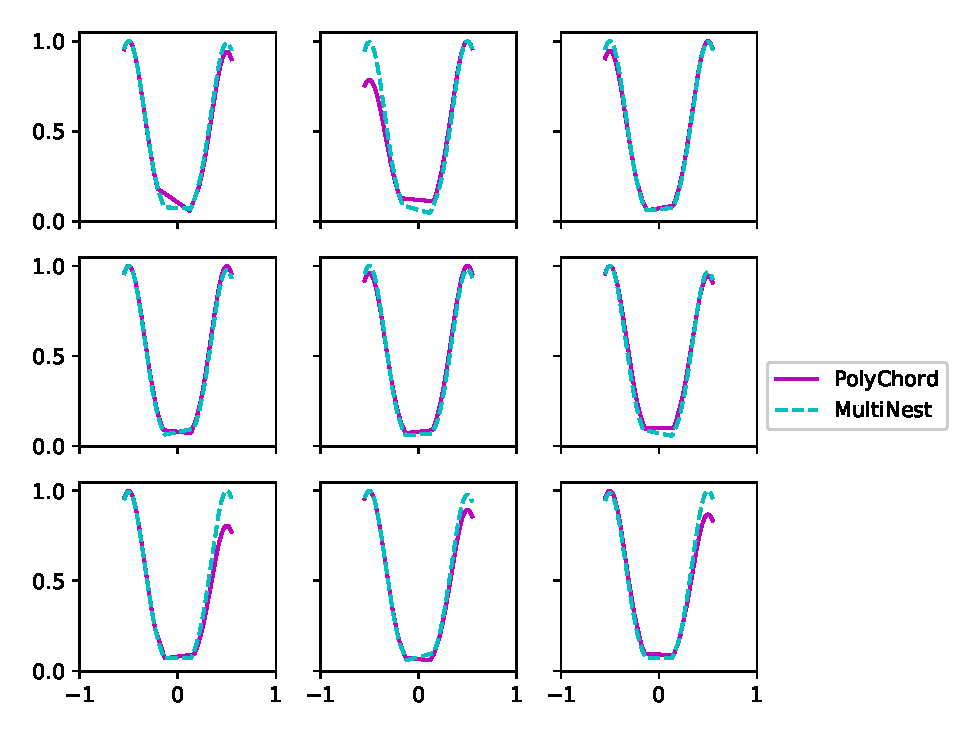
\includegraphics{polynestcomparison.eps}
  \caption{Posterior kernel density estimate plots for a double-Gaussian likelihood in 2D, showing the first parameter marginalised over the second, for both \texttt{PolyChord} and \texttt{MultiNest}. This is repeated nine times. \texttt{MultiNest} consistently produces peaks of equal height, while \texttt{PolyChord} fails to do so seemingly at random.}
  \label{fig:polynest}
\end{figure}

\newpage


\newpage

\section{CDT courses} 
As my funding is from the Centre for Doctoral Training, I attended several courses. In Michaelmas I attended Part III maths' \textit{Cosmology} and DAMTP's \textit{Introduction to Research Computing}, and in Lent Part III maths' \textit{Advanced Cosmology} and \textit{Astrostatistics}. In Michaelmas I also intended to attend \textit{Machine Learning for Fundamental Physics} in a partnership with the University of Munich, which was recorded in 2020. However, due to breaking my ribs in late October, I decided to leave this course for later to lighten my workload. I will attend this course over the summer once I have finished this report. I also plan to attend the second half of \textit{Cosmology} again for the same reason.

\textit{Introduction to Research Computing} has come in the most useful. As I began the year unfamiliar with Linux, the first few lectures was a good crash-course to translate the commands I knew from Windows PowerShell. As I was already very familiar with Python, the section on multiprocessing was the most useful element of the rest of the course. \textit{Astrostatistics} was helpful in reminding me that there are other sampling techniques besides \texttt{PolyChord}! It also covered the basics of Gaussian process modelling, which I discussed briefly in section \ref{sec:context}.

\newpage

\section{Computing}
A significant part of my learning this year has been gaining relevant computational skills. At the start of the year, I was comfortable using Windows, coding with my favourite editor Visual Studio Code. I was supposed to be provided with a MacBook, however this didn't arrive until early February. \texttt{PolyChord} is compatible only with Unix-based operating systems, so I wouldn't be able to learn how to use it on my Windows laptop. Therefore, I started using CSD3 (Cambridge Service for Data-Driven Discovery), a supercomputer accessed via SSH (secure shell). This overcame the compatibility issue with \texttt{PolyChord}, and was good practice for using the service. Initially I worked mainly using the login nodes, but these are intended to serve as an interface for submitting jobs to the compute nodes, which I would need to use to perform cosmological runs.

I have continued to use Visual Studio Code as my primary editor, as it has a \texttt{Remote - SSH} extension which allows near-seamless connection to a remote workspace. However, I found it limiting being unfamiliar with editing files directly in the terminal, as it is not convenient to have to create a VS Code workspace every time I want to edit a file. Therefore, I took some time to work through \textit{10-Minute Vim} to learn to use the editor \cite{vim}. I am starting to prefer using Vim keybindings, I use them in VS Code to edit text files, use \texttt{vimdiff} to compare git branches, and am using them in Overleaf right now!

I have used a range different programming languages over the years, but since the second year of my undergraduate degree I have almost exclusively used Python. The code I have worked with this year has been a mixture of pure Python and Python interfaces atop FORTRAN or C++ implementation. In December, I took part in the \href{https://adventofcode.com}{Advent of Code} using C++, which I chose over FORTRAN as I am familiar with curly-brace syntax from Java. I think it will be a useful exercise to do it again this year, but using FORTRAN \cite{advent}. 

I previously used git and github during my undergraduate degree, but only as the sole contributor to a project with two or three branches. This year I have learned about creating pull requests, and have become better at working on multiple branches and passing changes between them in both directions. I still feel I could be much better at collaborative development, but I am much more confident at changing existing code so I should get to practice collaboration much more.

CSD3 has three different types of Intel node. From oldest to newest: Skylake, Cascade Lake,  and Ice Lake. By default, a login session connects to a Skylake node, which used to submit jobs to the Cascade Lake compute nodes. This worked fine initially when I was only using \texttt{PolyChord}, but when I started probing the dark energy equation of state, \texttt{CAMB} suffered from segmentation-faults. I realised that I needed to load the Cascade Lake modules onto the login nodes to compile \texttt{CAMB} correctly for job submission. I realised a good way to remember the different installation steps would be to write bash scripts, as these would not only serve as a record but do it automatically when I needed to create a fresh Python virtual environment.

As a SL3 tier user, I can submit jobs on up to 8 nodes. Cascade Lake nodes have 56 cores, versus the 76 on Ice Lake. There are also Ice Lake login nodes, so there would be no compatibility issues between login and compute sessions. I intended to move over to Ice Lake, but I could not install the Planck likelihoods. I will try again once I have submitted this report.

\section{Conclusions}

Over the course of this year, I have become familiar with \texttt{PolyChord}, \texttt{Cobaya} and \texttt{CAMB}, both in using and modifying them. I have learned to use the supercomputer CSD3, both in terms of using Linux over SSH, and submitting large jobs to the compute nodes. 

I have found \texttt{PolyChord} to be a suitable way of fitting a \textit{linf}, a linear spline between either both a fixed number of nodes, and also allowing the number of nodes to vary as a parameter itself. However, when the number of live points (effective resolution) is increased to its recommended setting, it is unreliable in correctly identifying clusters. This became apparent when using a \textit{linf} to reconstruct the primordial matter power spectrum. I am working on adding a custom clustering argument to \texttt{PolyChord}, where the user can supply their own clustering algorithm.

The above was all intended as practice for investigating the dark energy equation of state parameter $w$. I have modified \texttt{Cobaya} to include an \texttt{external\_wa} option, analogous to \texttt{external\_primordial\_pk}, where the user supplies their own \texttt{cobaya.Theory} subclass to provide a table of $k$, $\mathcal P_\mathcal R(k)$ or $a$, $w(a)$ values. This change is almost complete, but understanding the clustering issue with \texttt{PolyChord} is vital before any definitive conclusions can be made about dark energy.

\section{Future Plans}
\subsection{Short term (less than three months)}
\begin{itemize}
  \item Watch the \textit{Machine Learning for Fundamental Physics} course and complete the exercises.
  \item Switch to the Ice Lake partition of CSD3. The current issue is getting \texttt{Cobaya} to install the Planck Likelihoods. The greater core count will allow runs to complete more quickly.
  \item Work out how to turn off non--linear lensing in \texttt{CAMB} via \texttt{Cobaya}, and see whether this recovers the right--hand mode in the primordial matter power spectrum. 
  \item Understand why \texttt{PolyChord} does not recover $N=4$ for the ``line" toy example.
  \item Finish testing \texttt{PolyChord} with custom clustering, and find a suitable replacement clustering algorithm.
  \item Work with Dr.~Handley to fix the issue where \texttt{PolyChord} is unable to produce a balanced posterior for a symmetric double Gaussian likelihood. We plan next to experiment with ideas from dynamic nested sampling.
  \item Understand why anesthetic is creating samples with NaN weights and likelihoods when using \newline \texttt{external\_wa}.
  \item Modify anesthetic to give a suitable warning when it encounters NaNs.
  \item Modify my \texttt{external\_wa} option in \texttt{Cobaya} so that it understands automatically that the parameters for the dark energy Theory are to be sampled with the rest of the cosmological parameters.
  \item Work through the \href{https://adventofcode.com}{Advent of Code}, but this time in FORTRAN \cite{advent}.
\end{itemize}
\subsection{Medium to long term (more than three months)}

\subsubsection{Tasks conditional on fixing and understanding \texttt{PolyChord}}

Once the different behaviour of \texttt{PolyChord} and \texttt{MultiNest} with multi-modal likelihoods has been understood, I will write this into an article. The custom clustering version of \texttt{PolyChord} will be merged into the master branch, and I will try and get the necessary changes to \texttt{Cobaya} also added to match, so that others may benefit from this analysis.

Once this is finished, and a suitable clustering algorithm has been chosen, I will finish reanalysing the primordial matter power spectrum. This may form a separate paper to the \texttt{PolyChord}--specific changes, as the improvements to non--linear lensing in \texttt{CAMB} which are responsible for the disappearance of the mode then it must also be demonstrated how to fix this.

Once I have finished studying the dark energy equation of state, it is only natural to probe the equations of state of the rest of the dark sector: dark matter and dark radiation, parameterised again by a linear spline. This will be less straightforward than for dark energy, as \texttt{CAMB} does not include options for varying the equation of state parameter for components other than dark energy. Therefore, I will need to modify both \texttt{CAMB} and \texttt{Cobaya} to add this feature. This work should form a suitable basis for another paper.

Once I have finished studying the dark energy equation of state, it is natural to probe those of dark matter, and the effective dark radiation proposed by W.E.V.~Barker discussed in section \ref{sec:barker}. The changes to \texttt{Cobaya} should be straightforward, as they will be very similar to the changes made to provide an external dark energy model. There are three paths I can take with the Boltzmann code:
\begin{enumerate}
  \item Modify \texttt{CAMB}. Until the Advent of Code, making changes to \texttt{PolyChord} is my only experience with FORTRAN, so I will find it most difficult to understand the existing code and where to make additions. However, this would be valuable experience, and the corresponding changes to \texttt{Cobaya} will be most straightforward.
  \item Switch to and modify \texttt{CLASS}. This is written in C++, which I have more experience in, and I am also used to the curly-brace syntax from Java in my first undergraduate year. However, I could find \texttt{CLASS} suffers from idiosyncrasies similar to non--linear lensing in \texttt{CAMB}. I am also not familiar with the \texttt{CLASS} interface in \texttt{Cobaya}.
  \item Switch to \texttt{PyCosmo} \cite{pycosmo}. This is an alternative Boltzmann code which generates efficient C/C++ code from \texttt{SymPy} (Symbolic Python). This represents a much faster way of adding the new components to the Boltzmann code. However, there is no interface for \texttt{PyCosmo} in \texttt{Cobaya}, which I would need to add myself. Its relative youth also means it lacks the decade(s) of testing of \texttt{CAMB} or \texttt{CLASS}.
\end{enumerate}
%
I will revisit this decision once the multi--modal issues with \texttt{PolyChord} have been resolved, and the priomoridal matter power spectrum and dark energy investigations are running.

\subsubsection{\texttt{anesthetic.2} and {Pandas}}

Dr.~Handley and Dr.~Hergt (a past member of the group) plan to \texttt{anesthetic.2} in the next few months. As well as performance improvements, they have updated the interface to more closely match that of \texttt{Pandas}, which \texttt{anesthetic} extends. I have found that some of the recent changes have had the side--effect of preventing some formatting parameters, such as the colour of a plot, to not be applied properly. I have corrected these issues by more closely following the structure of the overriden \texttt{Pandas} methods. However, this has led to me finding a bug in \texttt{Pandas} itself. Nested samples are weighted, which \texttt{Pandas} should be able to plot histograms and kernel density estimates out of the box. However, as discussed in section \ref{sec:de}, nested samples can contain NaN values, \texttt{Pandas} will drop when plotting. However, it cannot handle both weights and NaNs at the same time. I am working on a pull request, which will take several weeks to get merged first into the master branch, then months into the release version. Until this happens, I have provided a workaround by overriding the same methods in \texttt{anesthetic}.

By adding a new component with a dynamic equation of state to my analysis, I will be able to assess whether there is evidence to support a new component, 
A \textit{linf} can model both the periods before and after the transitions, and provide insight into the nature of the transition itself. As matter-radiation equality occurs at a redshift of around 3400 \cite{planck_6}, a \textit{linf} in $w_\textrm{dark radiation}(\log{a})$ would be more appropriate. 


As a part of this work, I would similarly like to look further back with the dark energy equation of state. Once I have successfully reproduced S.~Hee's results \cite{Sonke}, I will re-parameterise $w$ as $w(\log{a})$.

\subsection{Long term}

There are many other functions ripe for similar non-parametric reconstructions, for example the reionisation history $x_e(z)$, late--time matter power spectrum $P(k)$, CMB power spectra $C_\ell$ and lensing spectra $C_l^{\phi\phi}$. The 

\section{Acknowledgements}

Thank you to Cambridge Machines Access Management and Centre for Doctoral Training in Data Intensive Science for awarding the funding for my PhD.

\newpage
\emergencystretch=2em
\printbibliography
\end{document}
